%!TEX options = --shell-escape
\documentclass{tesisITAM}
\usepackage[utf8]{inputenc}
\usepackage{epstopdf,epsfig}  
\usepackage{hyperref}
\usepackage{apacite}
\usepackage{mathtools}
\usepackage{xcolor}
\usepackage{framed}
\usepackage{graphicx}
\usepackage{titlecaps}
\usepackage[font=bf]{caption}
\usepackage{rotating}
\usepackage{subfig}
\usepackage{multirow}
\usepackage{blindtext}
% \usepackage{minted}

\usepackage[toc,acronyms]{glossaries} 
% \makeglossaries
%!TEX root = ../main.tex
%%%%%%%%%%%%%%%%%%%%%%%%%%%%%%%% Acrónimos %%%%%%%%%%%%%%%%%%%%%%%%%%%%%%%%%%
% \newacronym[longplural={Frames per Second}]{fpsLabel}{FPS}{Frame per Second}
%%%%%%%%%%%%%%%%%%%%%%%%%%%%%%%%%%%%%%%%%%%%%%%%%%%%%%%%%%%%%%%%%%%%%%%%%%%%%

\newacronym{ITAM}{ITAM}{Instituto Tecnológico Autónomo de México}
% \newacronym{}{}{}
% \newacronym{}{}{}
% \newacronym{}{}{}
% \newacronym{}{}{}

%%%%%%%%%%%%%%%%%%%%%%%%%%%%%%%%% Términos %%%%%%%%%%%%%%%%%%%%%%%%%%%%%%%%%%%
\newglossaryentry{Linux}
{
  	name=Linux,
	    description={is a generic term referring to the family of Unix-like
                computer operating systems that use the Linux kernel},
  	plural=Linuces
}
	
\newglossaryentry{Wi-Fi}
{
	name = Wi-Fi,
	description = {Formalmente llamado IEEE 802.11, es un estándar de comunicación para redes locales inalámbricas}
}

%%%%%%%%%%%%%%%%%%%%%%%%%%%%%%%%% Símbolos %%%%%%%%%%%%%%%%%%%%%%%%%%%%%%%%%%%
% \newglossaryentry{pi}
%	{
%   	name={\ensuremath{\pi}},
%	    description={ratio of circumference of circle to its diameter},
%  		sort=pi
% 	}
%%%%%%%%%%%%%%%%%%%%%%%%%%%%%%%%%%%%%%%%%%%%%%%%%%%%%%%%%%%%%%%%%%%%%%%%%%%%%

% \loadglsentries{Aux_files/Glossary}


\mathtoolsset{showonlyrefs} 
% \loadglsentries[main]{Aux_files/Glossary}
% %!TEX root = ../main.tex
%%%%%%%%%%%%%%%%%%%%%%%%%%%%%%%% Acrónimos %%%%%%%%%%%%%%%%%%%%%%%%%%%%%%%%%%
% \newacronym[longplural={Frames per Second}]{fpsLabel}{FPS}{Frame per Second}
%%%%%%%%%%%%%%%%%%%%%%%%%%%%%%%%%%%%%%%%%%%%%%%%%%%%%%%%%%%%%%%%%%%%%%%%%%%%%

\newacronym{ITAM}{ITAM}{Instituto Tecnológico Autónomo de México}
% \newacronym{}{}{}
% \newacronym{}{}{}
% \newacronym{}{}{}
% \newacronym{}{}{}

%%%%%%%%%%%%%%%%%%%%%%%%%%%%%%%%% Términos %%%%%%%%%%%%%%%%%%%%%%%%%%%%%%%%%%%
\newglossaryentry{Linux}
{
  	name=Linux,
	    description={is a generic term referring to the family of Unix-like
                computer operating systems that use the Linux kernel},
  	plural=Linuces
}
	
\newglossaryentry{Wi-Fi}
{
	name = Wi-Fi,
	description = {Formalmente llamado IEEE 802.11, es un estándar de comunicación para redes locales inalámbricas}
}

%%%%%%%%%%%%%%%%%%%%%%%%%%%%%%%%% Símbolos %%%%%%%%%%%%%%%%%%%%%%%%%%%%%%%%%%%
% \newglossaryentry{pi}
%	{
%   	name={\ensuremath{\pi}},
%	    description={ratio of circumference of circle to its diameter},
%  		sort=pi
% 	}
%%%%%%%%%%%%%%%%%%%%%%%%%%%%%%%%%%%%%%%%%%%%%%%%%%%%%%%%%%%%%%%%%%%%%%%%%%%%%

\graphicspath{ {Figures/} }
\epstopdfsetup{outdir="Figures/"}


\title{Título}
\author{Autor}
\degree{Ingeniero en $\ldots$}
\advisor{Asesor}
\year{Año}
\setlength{\headheight}{13.1 pt}
%
% \glstoctrue

\colorlet{shadecolor}{blue!20}

\newcommand{\TODO}[1]{{\color{red}{ToDo: {#1}}}}
\newcommand{\NOTE}[1]{{\color{blue}{Note: {#1}}}}
\newcommand{\EXCISE}[1]{}

\renewcommand{\refname}{Referencias}

\begin{document}
	
	\maketitle
	\hypersetup{pageanchor=false}
	\publicationrights


	%%%%%%%%%%%%%%%%% Abstract %%%%%%%%%%%%%%%%%%%

	\begin{abstract}{english}
		\blindtext
	\end{abstract}

	% \begin{abstract}{english}
	% 	Abstract English
	% \end{abstract}

	\selectlanguage{spanish}
	
	\pagenumbering{roman}

	\tableofcontents
	\listoffigures
	\listoftables
	
	\newpage

	\pagenumbering{arabic}
	
	%%%%%%%%%%%%%%%%% Chapters %%%%%%%%%%%%%%%%%%%
	
	%!TEX root = ../main.tex
\chapter{INTRODUCCIÓN}
\label{ch:intro}

\section{Primera sección}
{\selectlanguage{english} \blindtext}



\subsection{Subsección}
{\selectlanguage{english} \blindtext}

\begin{itemize}
    \item First
    \item Second
    \item Third
\end{itemize}



	%!TEX root = ../main.tex
\chapter{MARCO TEÓRICO}
\label{ch2:MarcoTeorico}

\section{Acrónimos}
En el archivo auxiliar ``Aux\_files/Glossary.tex'' se definen los términos del glosario.
Es útil usar acrónimos: \gls{ITAM}. Si se usa por segunda vez ya no se expande: \gls{ITAM}. 

\section{Glosario}
Para usar un término del glosario: \gls{Wi-Fi}.

\section{Citas}
En el archivo auxiliar ``Aux\_files/FuentesConsultadas.bib'' se define la bibliografía. Se puede usar como: \cite{turing2009computing}.


\section{Imágenes}
Importar imágenes (con citas):

\label{robocup-ssl}
\begin{figure}
	\centering
		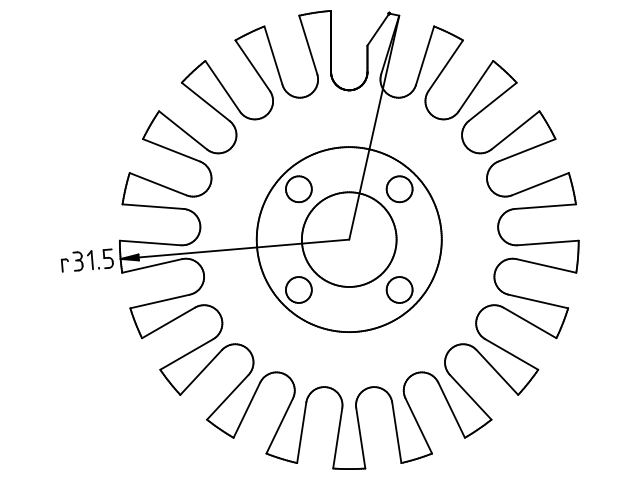
\includegraphics[width=.8\textwidth,height=.8\textheight]{rueda.png}
	\caption{Rueda Omnidireccional \protect\cite{itam-gary} }
	\label{fig:SP}
\end{figure}

Se pueden usar imágenes eps y ponerlas en página completa giradas.
\begin{sidewaysfigure}
	\centering
		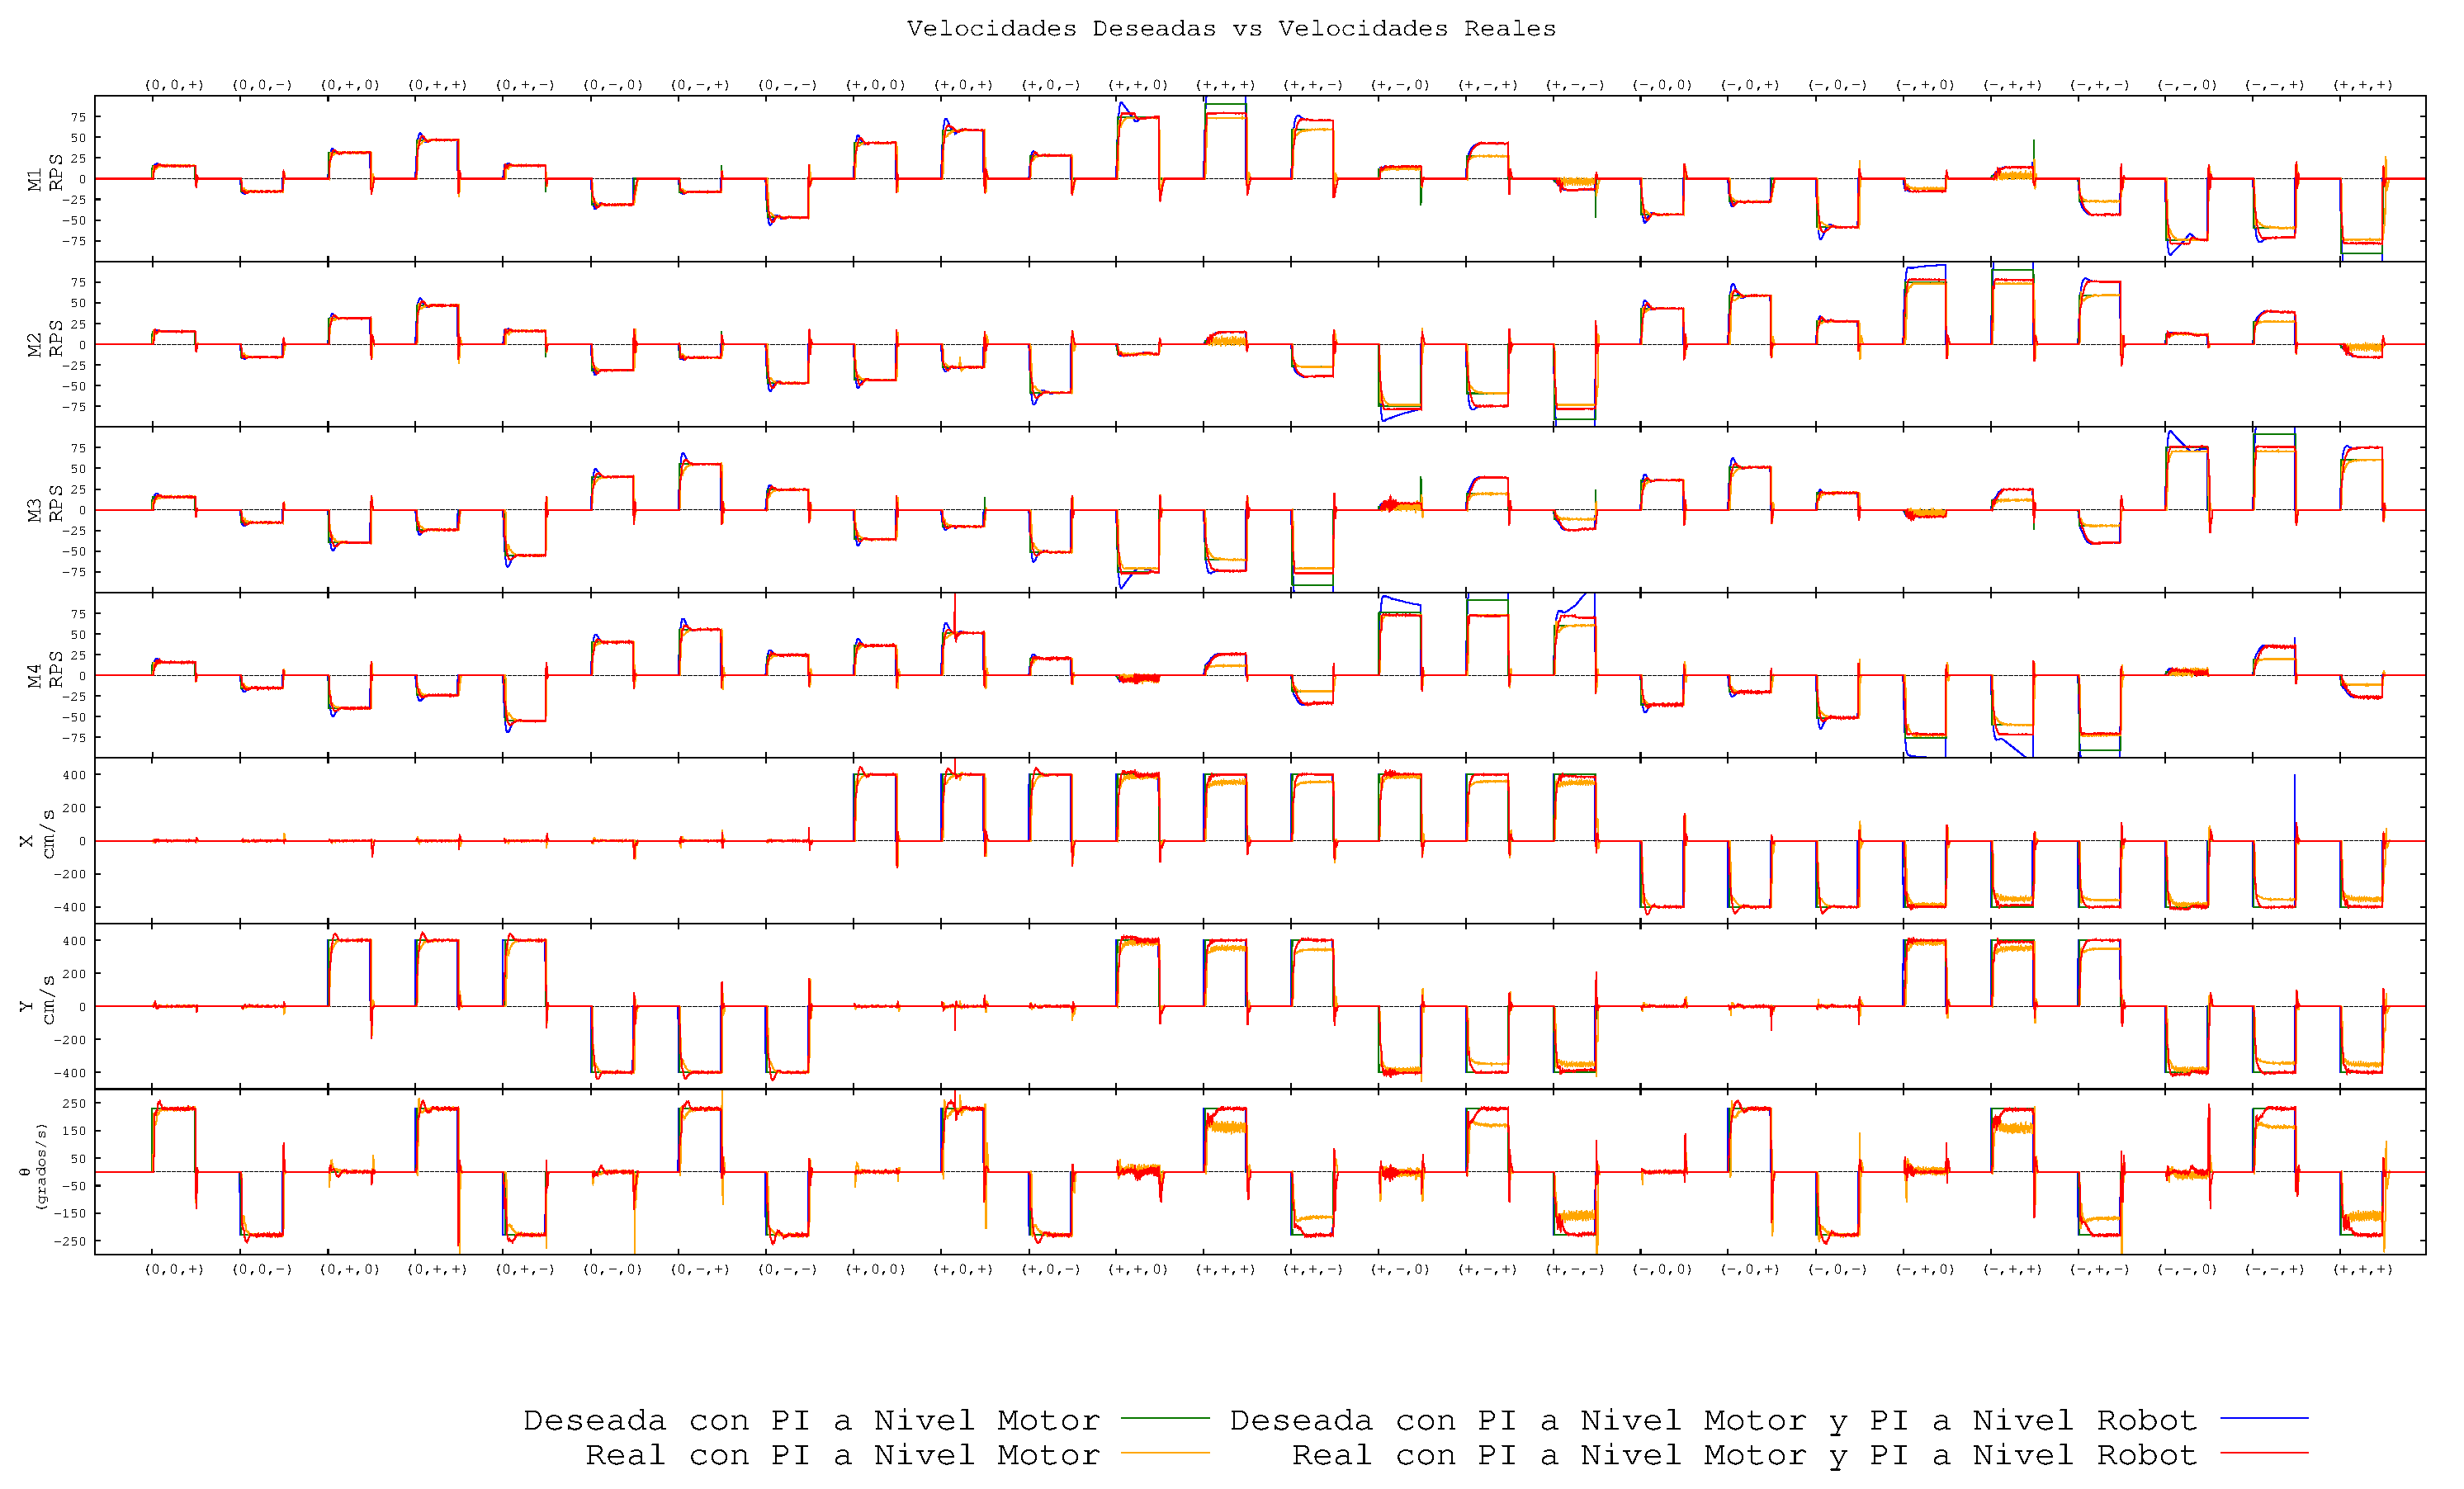
\includegraphics[width=\textwidth,height=0.9\textheight]{Figures/160517-vels-motVSmotrob_slide.eps}
	\caption{Velocidades Deseadas vs Velocidades Reales}
	\label{fig:vels_real_vs_des_mot}
\end{sidewaysfigure}





	%!TEX root = ../main.tex
\chapter{DISEÑO Y DESARROLLO DE UN ROBOT SSL}
\label{ch:disenio_y_des}
%\includegraphics[width=\textwidth]{diagArq.png}\\

% En general: descprición general de cada sección de DyDdP. Despues, una descripción específica de cada sección del robot.
En éste capitulo se presentan los resultados del diseño de un robot \gls{SSL} de acuerdo a la metodología de \textit{Diseño y Desarrollo de Producto} \cite{ulrich2009dise}. En el primer paso, \textit{Planeación}, se establecen las restricciones del producto y los objetivos que debe cumplir. En \textit{Desarrollo de Concepto} se prueba la viabilidad del uso de ciertas tecnologías mediante prototipos, para validar el concepto. En el tercer paso, \textit{Diseño a Nivel Sistema} se establece la arquitectura del producto definiendo los sistemas y componentes que lo conforman además de identificar interacciones y las interfaces entre los sistemas. El cuarto paso \textit{Diseño a Detalle} presenta el diseño final de los componentes de cada sistema y sus características. El quinto paso, \textit{Pruebas}, se presenta como parte del capítulo \ref{ch:res}.  
\EXCISE{
	\section {Planeación}
% Capítulos: 2, 3, 4, 5, 6, 7, 8, 9, 10, 15, 16, 17, 18
% Identificación de oportunidades abarcando la evaluación de los avances tecnológicos y los objetivos.
 % El resultado es la declaración de misión del proyecto que especifica el objetivo del producto, los supuestos básicos y las limitaciones. \par
% Producto de Plataforma


El robot está enfocado en la Plataforma existente de SSL: Visión especialmente \\
Se definió la arquitectura del sistema mostrada en la Fig. \ref{fig:diagArq}. \\
La arquitectura se realizó pensando el facilitar la modularidad. Facilitando la adaptación a otras aplicaciones así como poder modernizar por módulos cuando sea necesario. \\
Debido a que el robot, aunque independiente del sistema con el que se utilice, se valida con un sistema en específico (Robocup SSL), es importante incluir éste sistema dentro de la arquitectura. \\

\begin{figure}
	\centering
		\includegraphics[width=8cm]{diagArq.png}
	\caption{Arquitectura del Robot}
	\label{fig:diagArq}
\end{figure}
}
\EXCISE{
\subsection {Movimiento}
Se requiere movimiento omnidireccional para poder estar a la par de las capacidades de todos los equipos de Robocup SSL. \\
Para el movimiento omnidireccional, es necesario una rueda omnidireccional. \\
Es necesaria una rueda delgada \\
Rueda comercial: Mecanum, pero son muy anchas para esta aplicación \\
Es necesario diseñar y manufacturar una rueda propia que cumpla con las necesidades\\

\subsection {Pateo}
Existen dos tipos de pateo permitidos en SSL: straight y chip \\
Actualmente todos los equipos cuentan con ambos tipos de pateo \\
Dos posibilidades: neumático y eléctrico \\
El eléctrico ocupa menos espacio y se puede utilizar más veces sin recargar: aprendido de los TDP's de otros equipos \\
Son necesarios dos selenoides y un circuito de carga (con capacitor) que se autoregule \\
Dos tipos de Selenoides: comerciales y hechos en casa? \\
Se utiliza comercial por ser más eficiente aunque se pierde posibilidad de no ser cilíndrico y adaptarlo al espacio del robot \\
Se utiliza un sistema de palanca para poder tener un chip kicker \\
La primera generación de Eagle Knights con chip kicker \\

\subsection {Control de Pelota}
Es necesario para realizar un pateo eficiente \\
Escencial para mover la pelota cerca del robot \\
Por especificaciones de SSL, tiene que ser parelo al suelo \\
Los diseños de otros equipos utilizan motores brush con algún tipo de transmisión \\
Para el dribbler, se utilizan diversos tipos de espongas, material suaves \\

\subsection {Electrónica - Circuitos}
Se puede utilizar: FPGA, Microcontrolador, DSP, Computadora miniatura (Raspebbry Pi) y combinaciones \\

\subsection {Comunicación}
SSL permite cualquier tipo de comunicación inalámbrica excepto Bluetooth \\
Entre las opciones más populares estan: \gls{Wi-Fi}, Xbee, radios en otras frecuencias \\

\subsection {Energía}
Es necesario alimentar: Movimiento, Electrónica - Circuitos, Pateo, Comunicación \\



\subsection {ROS}
Debido a que se busca favorecer la modularidad en la totalidad del sistema, se decidió utilizar ROS \\
ROS se basa en módulos que se comunican entre sí, facilitando la escalabilidad y mejoramiento del sistema y los subsistemas. \\
}

% \subsection {Diseño}
% Considerar Plataforma y Arquitectura. \par
% Evaluar Nuevas Tecnologías. \par
% \subsection {Manufactura}
% Identificar restricciones de producción. \par
% Establecer estrategia para la Cadena de Suministro \par
% \subsection {Otras} 
% Investigación: Demostrar Tecnologías \par
% Dirección Gral: Asignar Recursos \par

\section {Planeación}

% Capítulos: 2, 5, 6, 7, 8, 9, 10, 11, 12, 14, 15, 16, 17, 18
% Se identifican las necesades del mercado objetivo
% se generan y evalúan conceptos alternativos del producto 
% uno o más conceptos se seleccionan para desarrollar
% pruebas adicionales, 
Se hace la planeación considerando las características de versiones previas y las especificaiones de la \gls{SSL}.
Las características de versiones anteriores del Robot para Robocup \gls{SSL} que se toman en cuenta en este diseño son:
\begin{itemize}
	\item Alta dependencia de manufactura externa, por no contar con el equipo necesario para realizar manufactura interna.
	% \item Alta dependencia de manufactura externa.\par Esto representa dificultad para realizar prototipaje además de elevar costos.
	\item Piezas frágiles, requiriendo ser reemplazadas frecuentemente durante pruebas y juegos. La rueda era uno de los componentes con mayores problemas.
	% \item Piezas frágiles. \par Se necesitaba reemplazar con alta frecuencia ciertas piezas, elevando costos.
	\item Tiempo de ensamblado elevado debido al número de piezas, impactando en los costos.
	% \item Tiempo de armado elevado. \par Producto de un elevado número de piezas únicas, además de elevar costos por requerir mayor material y manufactura.
	% \item Muchas piezas comerciales. \par Alta dependencia de terceros además de elevar los costos.
	% \item Difícilmente modificable. \par Una pieza cumplía múltiples funciones.
	\item Cómputo basado en un \gls{DSP} volviendo la programación compleja, difícil de parametrizar y modificar.
	\item No se tenía un diseño modular, haciendo difícil realizar modificaciones. 
	\item La carcasa no tenía el \gls{SP} integrado en su diseño, presentando problemas con la visión de la liga y siendo complejo modificar el \textit{id} de cada robot.
	\item Problemas en el sistema de energía, afectando particularmente a los motores. Estos requerían ser reemplazados frecuentemente tras descomponerse. Además de elevar costos, el tiempo de reemplazo era alto.

	% \item Mala integración con la visión de la liga. \par Las carcasas no se realizaban con un método de manufactura automatizado, provocando teniendo alto margen de error y problemas con el reconocimiento de cada robot por el sistema de visión de la liga.
\end{itemize}


En la sección \ref{robocup-ssl} se detallan las reglas y especificaciones que un robot debe cumplir para poder participar en Robocup \gls{SSL}. La solución debe cumplir con dichas especificaciones además de atacar los problemas detectados en versiones anteriores. Específicamente, el robot debe ser fácilmente modificable y de bajo costo, priorizando manufactura local.

Para poder mantener bajos costos y asumiendo que se tendrá una producción de pocas unidades, el método de \gls{MDF} resulta muy atractivo al contar en el laboratorio con el equipo adecuado. A pesar de ésto, no se pueden descartar otros métodos de manufactura ni utilizar piezas comerciales al proporcionar mayor calidad.


\section{Desarrollo de Concepto}
Para validar la viabilidad de utilizar \gls{MDF} como principal técnica de manufactura, se crearon dos prototipos utilizando piezas de versiones anteriores.

El primer prototipo se muestra en la Fig. \ref{fig:protoRob}). Tanto la base como la carcasa de cada motor se manufacturaron mediante \gls{MDF}. Mediante éste prototipo se validó la posibilidad de imprimir piezas de dimensiones similares a la base (150 mm de radio por 5mm de ancho). Aunque la base salió ligeramente dañada del proceso de \gls{MDF} por su tamaño, no afectó gravemente su estructura. Adicionalmente, con éste prototipo se pudo comenzar a probar el funcionamiento de los motores y el movimiento omnidireccional. Las ruedas utilizadas en el prototipo ocupan mucho espacio por lo que es necesario utilizar otras ruedas que ocupen menos espacio así como implementar un reductor de velocidad ya que se requiere menor velocidad de los motores y mayor torque. Por último, el motor debe ir elevado ya que de quedar cerca del suelo puede dañarse por la pelusa de la cancha.

El segundo prototipo se muestra en la Fig. \ref{fig:protoKicker}. El objetivo de éste prototipo fue validar si las piezas manufacturadas mediante \gls{MDF} se podían utilizar para el \gls{Kicker} sin que se dañasen rápidamente. Adicionalmente, se probó una primera versión del circuito de control. Las piezas funcionaron adecuadamente aunque la sujeción de las piezas presentó problemas debido a la fuerza ejercida por el selenoide.


\begin{figure}
	\centering
		\includegraphics[width=8cm]{proto_4}
	\caption{Prototipo del Robot}
	\label{fig:protoRob}
\end{figure}

\begin{figure}
	\centering
		\includegraphics[width=8cm]{proto_kicker_1}
	\caption{Prototipo del Kicker}
	\label{fig:protoKicker}
\end{figure}


\EXCISE{
	\subsection {Diseño}
	Investigar factibilidad de conceptos del producto \par
	Desarrollar conceptos de diseño industrial \par
	Construir y probar prototipos \par
	\subsection {Manufactura}
	Estimar costos \par
	Evaluar factibilidad de producción \par
	\subsection {Otras}
	Recabar necesidades \par
	Identificar Usuarios \par
	Identificar productos de la competencia \par
}
\section {Diseño a Nivel de Sistema}
% Capítulos: 2, 6, 10, 11, 12, 13, 14, 15, 16, 17, 18 
% Definir la arquitectura del producto 
% la descomposición del producto en subsistemas y componentes.
% Planes iniciales para el sistema de producción así como esquema de ensamble final para el sistema de producción. 
% Al final de esta fase se debe contar con:
	% un diseño geométrico del producto
	% una especificación funcional de cada uno de los subsistemas del producto
	% un diagrama de flujo preliminar del proceso para el ensamble final. 
% \EXCISE{
% 	\subsection {Diseño}
% 	Generar arquitecturas de producto. \par
% 	Definir subsistemas e interfaces principales. \par
% 	Refinar diseño industrial. \par
% 	Ingeniería preliminar de componentes. \par
% 	\subsection {Manufactura}
% 	Identificar proveedores para componentes clave. \par
% 	Efectuar análisis de fabricar contra comprar. \par
% 	Definir esquema final de ensamble. \par
% 	\subsection {Otras}
% 	Análisis de fabricar vs comprar \par
% }

Para realizar el Diseño a Nivel de Sistema, se identifican componentes funcionales que requiere la solución y se identifican las relaciones entre ellos para definir sistemas. Se presentan las interacciones incidentales entre los sistemas así como las interfaces entre sistemas. La arquitectura propuesta es modular, compuesta de seis sistemas.

% Se presenta una arquitectura modular con una funcionalidad específica para cada sistema que la compone: Chasis, Cómputo, Electrónica, Mecánica y Aditamentos para el Juego. \TODO{Cambiar...}

\subsection{Análisis de los Componentes del Robot}

%%%%%%%%%%%%%%%%%%%%%%%%%%%%%% BEGIN FIGURE %%%%%%%%%%%%%%%%%%%%%%%%%%%%%%
\begin{figure}
	\centering
		\includegraphics[width=\textwidth]{EKbot_Schematic.png}
	\caption{Esquemático: Elementos del Robot Omnidireccional}
	\label{fig:ekbot_schematic}
\end{figure}
%%%%%%%%%%%%%%%%%%%%%%%%%%%%%% END FIGURE %%%%%%%%%%%%%%%%%%%%%%%%%%%%%%
Para obtener una arquitectura modular, se identificaron 20 componentes necesarios de acuerdo a su función y se agruparon en 6 sistemas como se muestra en la Fig. \ref{fig:ekbot_schematic}, de los cuales dos son considerados críticos: Cómputo y Mecánica. 

\subsubsection{Chasis}
Componentes cuya función principal es proporcionar soporte estructural, protegiendo al resto de los sistemas ante colisiones. Está integrado por tres componentes: Base, Carcasa y Tapa. La función de la base es unir los sistemas mientras que la carcasa protege a los sistemas ante colisiones. La tapa implementa el \gls{SP} para ser compatible con los requerimientos de Robocup \gls{SSL}.

\subsubsection{Movimiento}
Sistema integrado por los componentes que le proporcionan movimiento en el mundo al robot. Está integrado por tres componentes: Actuador, Transmisión y Rueda. El actuador genera movimiento que se transmite mediante la transmisión a la rueda. Para obtener movimiento omnidireccional son necesarios por lo menos tres instancias de cada componente, por redundancia se utilizan cuatro. Por la funcionalidad que éste sistema proporciona es considerado crítico.

\subsubsection{Aditamentos de Apoyo}
Estos componentes son específicos para participar en juegos de Robocup \gls{SSL}. Un actuador, transmisión y rodillo son para el \gls{Dribbler} que retiene la pelota mientras que los otros dos sirven para patear la pelota. Para utilizar el robot en un contexto distinto a \gls{SSL}, éste es el sistema que se puede reemplazar.

\subsubsection{Energía}
Fuentes de corriente directa que alimentan a otros sistemas. Tanto el sistema de Movimiento como el de Aditamentos de Apoyo requieren 12V. El sistema de Cómputo requiere 5V.

\subsubsection{Drivers}
Componentes que sirven como interfaces entre sistemas. Se tienen 3 drivers, uno para cada tipo de actuador.

\subsubsection{Cómputo}
Los componentes del sistema se encargan de obtener, almacenar y procesar datos para generar y enviar señales de control a otros sistemas. Está compuesto de cinco componentes: Interfaz de Entradas/Salidas, Comunicación Inalámbrica, Función de Control, Velocímetro y Registros. El primero, sirve para comunicar componentes a través de distintos tipos de señales y protocolos de comunicación. La comunicación inalámbrica recibe datos de un sistema externo. La función de control calcula a partir de la información disponible la siguiente señal de control que aplicar a los actuadores del sistema mecánico. El velocímetro determina la velocidad real del robot mientras que la \gls{RAM} recibe datos de diversos componentes, los almacena y envía conforme son solicitados.

Se considera un sistema crítico debido a que el desempeño del robot está directamente relacionado a la frecuencia con la que éste sistema opere.





% \begin{enumerate}
% 	\item Chasis \par
% 		Componentes encargados de proporcionar soporte estructural, protegiendo al resto de los sistemas ante colisiones.
% 	\item Baterías \par
% 		Fuentes de corriente directa que alimentan a otros sistemas.
% 	\item Cómputo \par
% 		Obtener, almacenar y procesar datos para generar y enviar señales de control. 
% 	\item Drivers  \par
% 		Interfaces entre dos sistemas.
% 	\item Mecánica \par
% 		Integrado por los componentes que permiten el movimiento del robot en el mundo. 
% 	\item Aditamentos para el Juego \par
% 		Componentes específicos para participar en juegos de Robocup \gls{SSL}. 
% \end{enumerate}

\subsection{Interacciones entre Sistemas}
En la Fig. \ref{fig:incid_inter} se muestran las tres interacciones incidentales identificadas entre los distintos sistemas. La primera se da entre el chasis y los drivers, el calor generado por los drivers no se disipa rápidamente. La segunda es entre el chasis y las vibraciones generadas por la mecánica. La tercera se da al activar los componentes para el juego con la mecánica, pudiendo introducir errores en el movimiento del robot. 

Las interfaces entre los sistemas se muestran en la Fig. \ref{fig:interfaces_diag}. El sistema de baterías alimenta directamente al cómputo y a los drivers. El cómputo recibe señales del sistema mecánico y saca señales de control a los drivers que activan tanto el sistema mecánico como los aditamentos para el juego.
% A partir de la arquitectura, se realizó un análisis de las interacciones incidentales que pueden existir entre los distintos sistemas, mostrada en la Fig. \ref{fig:incid_inter}. Se identificaron tres interacciones incidentales. La primera es por el calor generado por la electrónica, especialmente por el circuito del kicker, con la carcasa al no permitir ventilación. La segunda se da por la vibración generada por los motores y ruedas, pudiendo afectar al chasis. La tercera interacción incidental se daría al activar la patada por la tercera ley de Newton. \par
% Adicionalmente, en la Fig. \ref{fig:interfaces_diag} se muestran las 3 interacciones deseadas entre los sistemas. La primera, entre Movimiento y Cómputo es bidireccional: se requiere de retroalimentación de Movimiento a Cómputo y de señales de control de Cómputo a Movimiento. La segunda se da del Computo a la Electrónica mediante señales de activación. La tercera se da de la Electrónica a los Aditamentos para la Pelota mediante señales eléctricas. \par
% Para el correcto funcionamiento del robot, son dos los sistemas críticos: movimiento y cómputo. El primero debido a que es el sistema que provee la característica omnidireccional al robot, mientras que el segundo es esencial para controlar eficazmente el movimiento del robot. Debido a ser sistemas críticos, un alto porcentaje del costo del robot debe pertenecer a estos. Como se busca crear un diseño de bajo costo, es en los otros sistemas que se debe buscar reducir el costo del robot. \par
\subsection{Arquitectura Propuesta}
En la Fig. \ref{fig:arq_rob} se muestra la arquitectura propuesta con los sistemas mencionados previamente así como los componentes de cada sistema y las interacciones existentes entre los componentes. A partir de los componentes de cada sistema, se puede comenzar a realizar el diseño a detalle de cada componente. Cada uno puede consistir de una o más piezas.


\begin{figure}
	\centering
		\includegraphics[width=\textwidth]{incidental_interactions}
	\caption{Interacciones Incidentales}
	\label{fig:incid_inter}
\end{figure}

\begin{figure}
	\centering
		\includegraphics[width=\textwidth]{Interfaces_interactions}
	\caption{Interacciones Deseadas}
	\label{fig:interfaces_diag}
\end{figure}

\begin{sidewaysfigure}
	\centering
		\includegraphics[width=\textwidth]{Arquitectura_ekbot.pdf}
	\caption{Arquitectura del Robot}
	\label{fig:arq_rob}
\end{sidewaysfigure}
% incidental_interactions  Interfaces_interactions Arquitectura_ekbot


\section{Diseño a Detalle}
% Capítulos: 11, 12, 13, 14, 15, 16, 17, 18
% Especificación completa de la geometría, materiales y tolerancias de todas las partes únicas del producto
% identificar las partes estandar a ser adquiridas de proveedores
% Al finalizar se debe contar con: 
	% documentación de control del producto: 
		% dibujos o archivos de la geometría de cada pieza
		% Especificaciones de piezas compradas
		% planes de proceso para la fabircación y ensamble del producto
% Terminar de definir: 
	% Selección de materiales
	% Costo de producción
	% Desempeño robusto del producto

En ésta sección se presentan los diseños finales obtenidos para cada componente de la arquitectura propuesta. Cada uno de los componentes son ensamblados con tornillos m3 de 5mm o 13mm de acuerdo a cada pieza. Cada componente puede estar compuesto por una o más piezas únicas. Con la finalidad de reducir costos, se prioriza utilizar como método de fabricación \gls{MDF} debido a que se cuenta con el equipo necesario. Para ello, se prioriza utilizar plástico \gls{ABS} por ser el de menor costo para ser usado en \gls{MDF} aunque se utiliza plástico \gls{HIPS} en las piezas de mayores dimensiones y que requieren mayor resistencia. Se utilizan piezas comerciales en los componentes donde se requiere alta precisión. El principal criterio de selección entre las alternativas de piezas comerciales es el costo, a menos que se trate de un sistema crítico, entonces se consideran otras características.

 % Para las piezas que necesiten ser comerciales, el principal criterio de selección es el precio a menos que pertenezcan a un sistema crítico, entonces se consideran otras características.
 % \TODO{Checar}
% Todas las piezas se pueden consutlar en \TODO{agregar liga}.

%%%%%%%%%%%%%%%%%%%%%%		CHASIS		%%%%%%%%%%%%%%%%%%%%%%
\subsection{Chasis}
Las piezas que comprenden éste sistema son las de mayores dimensiones, presentando dificultades para su manufactura por las características de dilatación del plástico \gls{ABS}. Para disminuir los problemas relacionados a manufacturar piezas grandes mediante \gls{MDF}, se utiliza plástico \gls{HIPS}. Aunque el plástico \gls{HIPS} tiene un costo superior al \gls{ABS}, se caracteriza por ser resistente a impactos, una característica deseada en la carcasa. Adicionalmente, permite manufacturar piezas de dimensiones mayores mediante \gls{MDF}, eliminando la necesidad de dividir las piezas en más pequeñas, facilitando el ensamblado. El modelo \gls{CAD} del sistema se muestra en la Fig. \ref{fig:chasis_cad}. 
% \TODO{checar, agregar total de piezas únicas}


\begin{figure}
	\centering
		\includegraphics[width=0.6\textwidth]{chassis_CAD}
	\caption{Chasis: Modelo CAD}
	\label{fig:chasis_cad}
\end{figure}
% \TODO{imagen del chasis real y cad}
\subsubsection{Tapa} 
La tapa consta de tres piezas únicas: dos diseños propios y tres imanes iguales con los que se ajusta al chasis facilitando el acceso a los componentes interiores. Una pieza cuenta con el \gls{SP}, lo cual facilita intercambiar los identificadores de cada robot. 

\subsubsection{Carcasa}
Compuesta de dos piezas únicas, su función principal es proteger al resto de los componentes ante posibles colisiones durante el juego y las pruebas. Una pieza se coloca al frente del robot, de la otra se utilizan tres y se colocan alrededor del robot ensambladas a la base. Se cuenta con orificios en las piezas para facilitar la ventilación para disipar el calor generado por los drivers.

\subsubsection{Base}
A ésta pieza se acoplan los demás sistemas así como la carcasa. Estructuralmente es una de las piezas críticas porque es el soporte de todos los componentes físicos.

\subsection{Energía}
Se utilizan dos modelos de baterías \textit{LiPo} distintas. Una batería de 7V para alimentar los componentes del Cómputo y al controlador del \gls{Dribbler}. Dos baterías de 12V alimentan a un controlador cada una. Específicamente, una alimenta a los drivers de los motores y la otra al controlador del \gls{Kicker}. El conector de la batería de 7V es distinto al de las baterías de 12V para evitar conectarlas a los sistemas erróneos. Utilizando una batería de 900mAh para la alimentación de los motores, el mínimo tiempo de uso esperado es de 6.75 minutos si los motores se encuentran a la máxima velocidad. El tiempo es el mismo para el \gls{Kicker} si el consumo de éste fuera el máximo de manera continua. 




%%%%%%%%%%%%%%%%%%%%%%%  Mecánica   %%%%%%%%%%%%%%%%%%%%%%%%%%%
\subsection{Movimiento}
El sistema mecánico está conformado por tres componentes, requiriendo cuatro \textit{instancias} de cada componente. Todas las piezas no comerciales están manufacturadas mediante \gls{MDF} utilizando plástico \gls{ABS} para reducir costos.
% \TODO{Agregar imagen del sistema cad y real}

\subsubsection{Motor}
Se utiliza un motor sin escobillas Maxon 200142 \cite{maxon_motor} que cuenta con tres sensores hall. El motor se acopla al chasis mediante una pieza propia. Motores de ésta marca han sido utilizados ampliamente por otros equipos de \gls{SSL} ya sea éste modelo o similares; estos motores habían sido previamente adquiridos para una generación anterior de los robots pero no fueron utilizados. Con la finalidad de reducir costos, se optó por utilizar estos motores en lugar de comprar nuevos. Los motores constituyen el componente más caro del robot (por necesitar cuatro) pero a la vez son uno de los componentes críticos ya que se requiere de motores eficientes, de tamaño reducido y que cuenten con retroalimentación para realizar control a lazo cerrado. En la Fig. \ref{fig:mot_trans_cad} se muestran acoplados éste componente y la transmisión.

\begin{figure}
	\centering
		\includegraphics[width=0.6\textwidth]{motor_trans_CAD}
	\caption{Motor y Transmisión: Modelo CAD}
	\label{fig:mot_trans_cad}
\end{figure}


\subsubsection{Transmisión}
Para acoplar el motor a la rueda se utiliza un tren de engranes rectos con reducción de velocidad de 3.5. Se optó por utilizar piezas comerciales debido a que se trata de un componente que requiere alta precisión para un acoplamiento adecuado. Se utilizan engranes rectos ya que, aunque éste tipo de engrane ocupa mayor espacio respecto a engranes planetarios, son más baratos. Al motor se acopla mediante un prisionero el \textit{pinion} \cite{pinion}. La rueda se acopla a un \textit{hub} \cite{dual_ball_bearing} al cual también se acopla el engrane \cite{gear_motor}.  Se utiliza como eje un tornillo de $\frac{1}{4}^{\prime\prime}$ el cual se introduce en el \textit{hub} y en \textit{motor\_hub}. Son necesarios dos separadores para ajustar la rueda a la altura del eje adecuada.

\subsubsection{Rueda}
La rueda consiste en cuatro piezas únicas: la silueta, rodillo, o-ring \cite{o-rings} y un cable. La silueta  (Fig. \ref{fig:ruedaOmni} \subref{rueda_silueta}) es la pieza principal de la rueda, está manufacturada mediante \gls{MDF}. Se utilizan 21 rodillos a los cuales se les coloca un o-ring a cada uno. Mediante el cable, se insertan los rodillos a la silueta.
En la Fig. \ref{fig:ruedaOmni} \subref{rueda_cad} se muestra el ensamble en CAD de la rueda. 
En la Fig. \ref{fig:ruedaOmni} \subref{exploded_assembly} se muestran las 4 piezas únicas utilizadas en la rueda, en orden descendiente: o-ring, rodillo, cable y silueta.

% \TODO{Agregar imagen de todo el sistema}
\begin{figure}%
	\centering
		\subfloat[Diagrama de la silueta]{{ 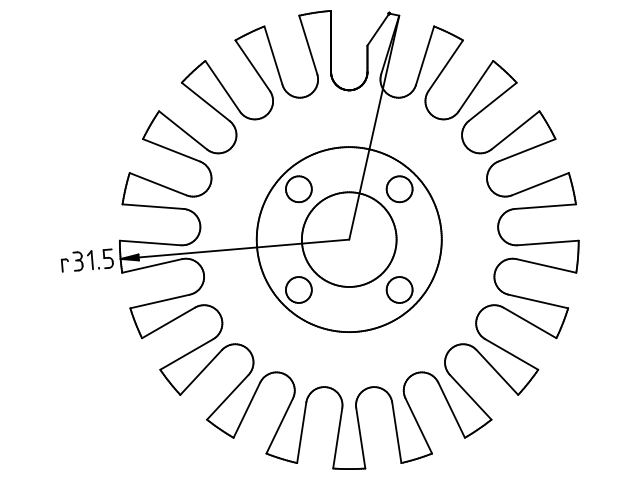
\includegraphics[width=0.4\textwidth]{rueda.png} \label{rueda_silueta} }}%
		\qquad
		\subfloat[Modelo CAD del componente]{{\includegraphics[width=0.3\textwidth]{rueda_CAD.png} \label{rueda_cad} }}%
		\qquad
		\subfloat[Piezas que conforman la rueda]{{\includegraphics[width=0.4\textwidth]{ruedaAssembly.png} \label{exploded_assembly} }}%
		\qquad
	\caption{Rueda Omnidireccional Utilizada}
	\label{fig:ruedaOmni}%
\end{figure}

%%%%%%%%%%%%%%%%%%%%%%%%%%%   ADITAMENTOS   %%%%%%%%%%%%%%%%%%%%%%%%%%%
\subsection{Aditamentos de Apoyo}
Este sistema es específico para participar en juegos de Robocup \gls{SSL}. Éste sistema se puede reemplazar si el robot es utilizado para otra aplicación.
El sistema está compuesto de cinco componentes, agrupados en dos subsistemas: \gls{Dribbler} y \gls{Kicker}. Los únicos componentes comerciales son actuadores: un motor con escobillas para el \gls{Dribbler} mientras que para el \gls{Kicker} es necesario utilizar selenoides comerciales. Para ambos casos el precio fue el principal factor de selección.

\subsubsection{Kicker}
El objetivo de éste componente es patear la pelota.
Se utiliza un selenoide como componente principal y un total de cuatro piezas únicas manufacturadas mediante \gls{MDF} para acoplar el componente al chasis. Otra pieza se acopla al selenoide para realizar el pateo de la pelota.
En la Fig. \ref{fig:cad_kicker} se muestra el modelo \gls{CAD} del kicker.

\begin{figure}
	\centering
		\includegraphics[width=0.5\textwidth]{kicker_assembly}
	\caption{Kicker: Modelo CAD}
	\label{fig:cad_kicker}
\end{figure}

\subsubsection{Dribbler}

El dribbler permite mantener al robot mantener la posesión de la pelota.
Está compuesto de tres subcomponentes: motor, transmisión y rodillo. Se utiliza un motor con escobillas \cite{dribbler_motor} debido a que no se requiere un control preciso de velocidad. Como transmisión se utiliza un tren de dos engranes manufacturados mediante \gls{MDF} debido al bajo torque que se requiere. En la Fig. \ref{fig:dribbler_cad} se muestra el modelo \gls{CAD} de éste componente así como el componente acoplado al robot.

\begin{figure}
	\centering
		\subfloat[Modelo CAD]{{ \includegraphics[width=0.4\textwidth]{dribbler_CAD} }}
		\qquad
		\subfloat[Acoplado al robot]{{ \includegraphics[width=0.4\textwidth]{dribbler_real} }}%
		\qquad	
	\caption{Dribbler}
	\label{fig:dribbler_cad}
\end{figure}


%%%%%%%%%%%%%%%%%%%%%%%%%%%   DRIVERS   %%%%%%%%%%%%%%%%%%%%%%%%%%%
\subsection{Drivers}
Éste sistema es la interfaz entre el sistema de cómputo y los actuadores. Es necesaria una interfaz debido a que el cómputo utiliza baja potencia mientras que los actuadores utilizan alta potencia. La mayoría de las piezas utilizadas en éste sistema son comerciales al tratarse de componentes eléctricos. Además de priorizar la reutilización de componentes se quiere minimizar el costo. El sistema también cuenta con piezas no comerciales manufacturadas con \gls{ABS}. La función de éstas piezas es de acoplamiento.

\subsubsection{Controlador de Motores}
Como interfaz entre el subsistema de \textit{Cómputo} y los motores sin escobillas que actuan las ruedas, se utilizan un \gls{ESC} \cite{esc_afro} por motor. Cada \gls{ESC} recibe una señal \gls{PWM} que codifica la velocidad deseada a 50 Hz, el ancho del pulso va de 1ms a 2ms, siendo 1.5ms la posición neutral. 

\subsubsection{Controlador Kicker}
El circuito está compuesto de cuatro subsecciones: carga, almacenamiento, detección de la pelota y activación. La carga se encarga de incrementar 12 V de voltaje de entrada a 200 V y mantenerlos, pasándolos al almacenamiento que consiste en un capacitor de 1000 $\mu F$. La detección de la pelota consiste en un diodo infrarrojo y un fotodiodo que activan un relevador si se detecta un objeto entre ambos. La subsección de activación recibe la señal de la \gls{FPGA}, estando aislada eléctricamente mediante octocopladores. El circuito se muestra en la Fig. \ref{fig:circuito_kicker}.

\begin{figure}
	\centering
		\includegraphics[width=\textwidth]{circuito_kicker}
	\caption{Circuito para el Kicker}
	\label{fig:circuito_kicker}
\end{figure}



\subsubsection{Controlador Dribbler}
El controlador del \gls{Dribbler} utiliza un puente H \cite{instruments2005l293} para dar energía al motor además de un regulador de voltaje que entrega 5 V a la salida. 


%%%%%%%%%%%%%%%%%%%%%%%%% Cómputo %%%%%%%%%%%%%%%%%%%%%%%%
\subsection{Cómputo}
Está compuesto por un XBee WiFi y una tarjeta de desarrollo \textit{Mojo} \cite{embedded_micro} la cual integra una \gls{FPGA} y un microcontrolador \gls{AVR}. 

% \NOTE{se podría agregar imágen de interacciones e interfacez entre Cómputo con electrónica}
% \subsubsection{\gls{FPGA} }
En la Fig. \ref{fig:arq_fpga} se muestra la arquitectura implementada en la FPGA así como los protocolos de comunicación usados entre la FPGA y los otros componentes. Los procesos implementados en la FPGA buscan aprovechar la alta frecuencia a la cual opera. Además, al no ser secuencial se pueden tener el número necesario de entradas y salidas operando de forma simultánea. En cambio, utilizar un mictrocontrolador \gls{AVR} facilita la implementación de las operaciones necesarias para realizar algoritmos de control así como realizar cálculos matriciales.
Aunque la tarjeta \textit{Mojo} representa un alto porcentaje del costo, al tener integradas una \gls{FPGA} y un \gls{AVR} ofrece características que son de gran utilidad como el manejo en paralelo de múltiples entradas y salidas. 

\begin{figure}
	\centering
		\includegraphics[width=\textwidth]{FPGA_model}
	\caption{Modelo Implementado en la FPGA}
	\label{fig:arq_fpga}
\end{figure}
% \TODO{agregar la parte de AVR ???}
\subsubsection{Comunicación Inalámbrica}

Para la comunicación inalámbrica se utiliza un XBee \gls{Wi-Fi} el cual recibe el vector $(X, Y, \theta)$ de velocidad deseada del robot además de comandos para los aditamentos. Se utiliza direccionamiento estático y mensajes UDP para evitar retransmisiones. Cada mensaje utiliza 12 bytes que codifican el vector velocidad del robot $(X, Y, \theta)$ y la acción deseada para los aditamentos de apoyo.
% Componente encargado de interactuar con el sistema externo. Recibe un vector $(X, Y, \theta )$ además del comando para los aditamentos. Los datos se los pasa al subcomponente \textit{Cómputo}. Esta compuesto por una targeta Xbee \gls{Wi-Fi} \cite{xbee_wifi}. Los datos son recibido mediante el protocolo UDP ya que solamente se requiere el último dato disponible y se evitan retransmiciones en caso de pérdida de los paquetes.

\subsubsection{Interfaz de Entrada/Salida}

Se tiene tres posibles fuentes de entrada: la comunicación inalámbrica, sensores hall de los motores y el \gls{AVR}. Para la comunicación inalámbrica es necesaria una interfaz \gls{UART} mientras que para el \gls{AVR} se utiliza una interfaz \gls{SPI}. Se utiliza una cola para guardar los datos provenientes del AVR y otra para los de la comunicación inalámbrica. Las señales de los sensores Hall se pasan al velocímetro. 

Existen cinco salidas a distintos componentes. Para la salida al \gls{AVR} se utiliza la interfaz \gls{SPI} y para la comunicación inalámbrica la interfaz \gls{UART}. Tanto para la salida a los drivers de motores como del \gls{Dribbler} se utiliza un módulo que convierte el dato a una señal \gls{PWM}. Por último, la salida al controlador del \gls{Kicker} es binaria.

% Para las salidas, se tiene una máquina de estados que de acuerdo a prioridades previamente asignadas, lee de los registros para establecer la señal adecuada en cada salida. La prioridad más alta la tiene el \gls{AVR}, la segunda el controlador de los motores, después los drivers de kicker y dribbler, por último el \gls{Wi-Fi}.

\subsubsection{RAM}
La \gls{RAM} se implementó mediante registros de 8 bits con direccionamiento de 7 bits; la lectura y escritura son independientes. Para la escritura se utiliza un esquema \textit{Round Robin} que toma datos de las colas asociadas al \gls{AVR} y a la comunicación inalámbrica así como del velocímetro. 

Para la lectura se utilizan prioridades en caso de que dos componentes soliciten leer registros en el mismo ciclo de reloj. La prioridad más alta se asignó al \gls{AVR}, la segunda al controlador de los motores, después a los drivers de \gls{Kicker} y \gls{Dribbler}, por último al \gls{Wi-Fi}. 
Las prioridades están pre-codificadas en la FPGA, se definieron de acuerdo a la importancia de los procesos que solicitan los datos.
% Las prioridades están \textit{hard-coded} en la FPGA, se definieron de acuerdo a la importancia de los procesos que solicitan los datos.

\begin{table}
\centering
\caption{Secuencia de los Sensores Hall por Motor}
\begin{tabular}{l|c c c }

 & $H^1$ & $H^2$ & $H^3$  \\
\hline
1   & 0 & 0 & 1\\
2   & 0 & 1 & 1\\
3   & 0 & 1 & 0\\
4   & 1 & 1 & 0\\
5   & 1 & 0 & 0\\
6   & 1 & 0 & 1\\
% \hline
% \multicolumn{3}{c}{Datos en RPS}
\end{tabular}
\label{table:hall_seq}
\end{table} 

\subsubsection{Velocímetro}
El cálculo de las velocidades reales de cada motor se realiza a partir de las tres señales de retroalimentación de los motores. La Tabla \ref{table:hall_seq} muestra la secuencia seguida cada $ \frac{1}{8} $ de revolución. Utilizando un contador por motor, se incrementa con cada cambio de las señales de los sensores Hall. Cada tiempo $t$ constante, el valor del contador se escribe a registros y el contador se establece en 0. Manteniendo la última señal de dos sensores hall por motor, la dirección del motor se detecta mediante la función lógica $ H_{t}^1 \oplus H_{t-1}^2 $.





% FPGA_model

\subsubsection{Ciclo de Control}



% En el microcontrolador se calcula la velocidad deseada de cada motor en el siguiente ciclo utilizando la velocidad de robot deseada y las velocidades reales de los motores. El vector de velocidades de motor deseadas se envía a la \gls{FPGA}, componente que aplica las señales de salida pertinentes.
El microcontrolador calcula y envía a la \gls{FPGA} la señal de control deseada para cada motor. Cada señal de control es la salida de un lazo de control PI a nivel motor  utilizando el error en la velocidad por motor. Las variables del control PI son calculadas manualmente. De la FPGA se obtienen, por motor, los pulsos de los sensores hall $p_t$ contados en una ventana de tiempo $F_m (hz)$. Conociendo los pulsos que genera cada motor por revolución $p_r$ se obtiene la velocidad real de cada motor mediante la ecuación \eqref{eq:vel_real_mots}. Las velocidades de motor deseadas se obtienen a partir de un vector de velocidades de robot deseadas mediante la ecuación \eqref{eq:velsMots_vals} utilizando los valores mostrados en la Fig. \ref{fig:angs_vals}.

\begin{gather}
	v_r = \frac{\left( p_t \right) \left( F_m \right) } { p_r} \label{eq:vel_real_mots}
\end{gather}

% Mediante la ecuación \eqref{eq:velsMots_vals} se obtiene el vector de velocidades de motor deseadas a partir de un vector de velocidades deseadas del robot. 

\begin{gather}
	% v_{x}^{'} = \frac{ v_x \cdot e } { 2 \pi r} \label{eq:reductorPerim}\\
	% v_1 = v_x \sin\varphi_1 + v_y\cos\varphi_1 + R \omega \label{eq:velMot1}\\
	v_m^d = 
		\left(\begin{array}{c}
			v_1 \\ v_2 \\ v_3 \\ v_4 
		\end{array}\right)
		= 
		\begin{bmatrix}
			+0.8090 & +0.5878 & 1 \\
			-0.8090 & +0.5878 & 1 \\
			-0.6691 & -0.7431 & 1 \\
			+0.6691 & -0.7431 & 1 \\
		\end{bmatrix}
		\left(\begin{array}{c}
			v_x^{'}  \\ v_y^{'}  \\ {85 w}^{'} 
		\end{array} \right) \label{eq:velsMots_vals} \\
		% v_d = D V_{d}^{'} \label{eq:velsMotsReduce} \\
\end{gather}

\begin{figure}
	\centering
		\includegraphics[width=\textwidth]{ang_rob_vals}
	\caption{Diagrama del modelo implementado}
	\label{fig:angs_vals}
\end{figure}

 % a partir de la ecuación \eqref{eq:velsMotsReduce}
La velocidad real del robot se puede calcular definiendo \( D^{+} \) como la pseudoinversa de $D$ (definida en la ecuación \eqref{eq:velsMotsReduce}) tal que la ecuación \eqref{eq:DsToIdent} se cumple. Definiendo el vector \( v_{r} = \begin{pmatrix}v_1^{r} & v_2^{r} & v_3^{r} & v_4^{r} \end{pmatrix}^{T} \) de velocidades reales de motor se obtiene \eqref{eq:velsMotToVelsRob} donde $V_r$ es el vector de velocidades reales del robot.

\begin{gather}
	D^{+}D = I_3 \label{eq:DsToIdent} \\
	V_{r} = D^{+}v_r \label{eq:velsMotToVelsRob} \\
\end{gather}

Es necesario encontrar la matriz \( D^{+} \), para el caso específico \(  \varphi_1 = \varphi_2 \) y \(  \varphi_3 = \varphi_4 \), la pseudoinversa se define en \eqref{eq:pseudo_inv}. A partir  de los vectores de velocidades reales y deseadas del robot se obtiene el error utilizado en el segundo lazo de control PI. El esquema completo de control se muestra en la Fig. \ref{fig:ciclos_ctrl_avr}.

\begin{gather}
	D^{+} = \begin{bmatrix}a & -a &-c & c \\e & e & -g & -g \\ i & i & k & k \end{bmatrix} \\
	\label{eq:pseudo_inv} \\
% \end{gather}
% \begin{gather}
	\begin{aligned}
	a & = c \cdot \cos 54  & \qquad k & = \frac{1}{\frac{2\cos 42}{\cos 54} + 2} \\
	c & = \frac{1}{\frac{2 (\cos 42)(\sin 54) }{\cos 54} + 2\sin 42} & e & = \frac{1}{2(\cos 54 + \cos 42)} \\ 
	i & = \frac{k \cdot \cos 42}{\cos 54} & g & = e \\
	% \end{split}
% \end{gather}
% \begin{gather}
	% \begin{split}
	% k & = \frac{1}{\frac{2\cos \varphi_3}{\cos \varphi_1} + 2} \\
	% e & = \frac{1}{2(\cos \varphi_1 + \cos \varphi_3)} \\
	% g & = e \\
	\end{aligned}
\end{gather}

\begin{figure}
	\centering
		\includegraphics[width=\textwidth]{ciclo_ctrl_avr}
	\caption{Ciclos de Control implementados en el AVR}
	\label{fig:ciclos_ctrl_avr}
\end{figure}


Antes de calcular la señal de control, se leen de la \gls{FPGA} tanto las velocidades de motor reales como las de robot deseadas. El ciclo de control se ejecuta a una frecuencia constante, determinada por una interrupción de reloj en el microcontrolador. Para mantener la sincronía, la señal de control calculada en cada ciclo se envía al inicio del siguiente ciclo. En la Fig. \ref{fig:funcs_avr} se muestra la secuencia de funciones implementadas en el microcontrolador.

\begin{figure}
	\centering
		\includegraphics[width=\textwidth]{avr_seq}
	\caption{Secuencia de Funciones en el microcontrolador}
	\label{fig:funcs_avr}
\end{figure}



% La secuencia de funciones realizadas por el microcontrolador se muestra en la Fig. \ref{fig:funcs_avr}. Por sincronía, se inicia el ciclo enviando la señal de control del ciclo anterior a la FPGA. Después, se leen de la FPGA tanto las velocidades reales como las deseadas las cuales se utilizan en un ciclo de control PI para calcular el vector $(X^\prime, Y^\prime, \theta^\prime)$ de velocidades deseadas. A partir de éste vector se calcula el vector $V_m$ de velocidades de motor deseadas al cual se le aplica un ciclo de control PI para obtener el vector $V_m^\prime$ el cual se envía a la FPGA para ser aplicado. El ciclo se realiza cada tiempo $t$ constante, mediante una señal de interrupción generada por el reloj del \gls{AVR}.




% En la Fig. \ref{fig:angs_vals} se muestra el diagrama con los valores utilizados para la implementación. A partir de un vector $V_d$ de velocidades deseadas del robot, dados los ángulos definidos, mediante la ecuación \eqref{eq:velsMots_vals} se obtiene el vector de velocidades deseadas de motor $v_m^d$. Utilizando éste vector y el de velocidades de motor reales $v_r$ se puede obtener el error por motor utilizado en el primer lazo de control PI.
 % que recibe de entrada el primer lazo de control PI. 








% , es posible calcular la velocidad real \( v_{r} \) a la cual se está moviendo cada motor. Definiendo el error como $v_e = v_{d} - v_{r}$ por cada motor, se puede aplicar un control PI de acuerdo a la eq. \ref{eq:ctrl_PI}.  


% \begin{gather}
% 	k_p e(t) + k_i \int_{0}^{t}e(\tau)d\tau  \label{eq:ctrl_PI} \\
% \end{gather}

% \subsubsection{PI a Nivel Robot}
% \label{subsubsec:PI_ROBOT}


% La velocidad real del robot se puede calcular a partir de la ecuación \eqref{eq:velsMotsReduce}, definiendo \( D^{+} \) como la una pseudoinversa de $D$ tal que la identidad \eqref{eq:DsToIdent} se cumple. Definiendo el vector \( v_{r} = \begin{pmatrix}v_1^{r} & v_2^{r} & v_3^{r} & v_4^{r} \end{pmatrix}^{T} \) se obtiene la identidad \eqref{eq:velsMotToVelsRob}. 


% \begin{gather}
% 	D^{+}D = I_3 \label{eq:DsToIdent} \\
% 	V_{r} = D^{+}v_r \label{eq:velsMotToVelsRob} \\
% \end{gather}

% Para determinar el vector de velocidades reales del robot, es necesario encontrar la matriz \( D^{+} \). Para el caso específico en el que \(  \varphi_1 = \varphi_2 \) y \(  \varphi_3 = \varphi_4 \), la pseudoinversa se define en \eqref{eq:pseudo_inv}. Utilizando el vector de velocidades reales del robot se obtiene el error utilizado en el segundo lazo de control PI. El esquema completo de control se muestra en la Fig. \ref{fig:ciclos_ctrl_avr}.

 % El segundo lazo de control PI utiliza el error en la velocidad del robot obteni




% Obteniendo el error $V_e = V_d - V_r$, se puede implementar un control PI (eq. \ref{eq:ctrl_PI}).

% La señal de control es calculada mediante dos ciclos cerrados donde se aplica un algoritmo PI en cada uno como se muestra en la Fig. \ref{fig:ciclos_ctrl_avr}. El ciclo primer ciclo se realiza a nivel de motor utilizando el error de la velocidad de cada motor. Para el segundo ciclo, se calcula el vector de velocidades reales $( X, Y, \theta )$ mediante la matríz de acoplamiento inversa y se obtiene el error. 


% Primero, un control PI determina un vector V ′ que se ma- l
% pea a las velocidades de motor deseadas Vm. A continuacio ́n, se aplica un segundo control PI a cada motor cuya salida se env ́ıa a la FPGA para convertirla a una sen ̃al PWM y alimentarla al ESC correspondiente. La velocidad real de cada motor se lee de la FPGA como retroalimentacio ́n del segundo ciclo de control. Adicionalmente, utilizando la matriz de acoplamiento inversa se obtiene el vector de velocidades reales (X′ ,Y′ ,θ′) que utiliza el primer control PI.






% \begin{figure}%
%     \centering
%     \subfloat[label 1]{{\includegraphics[width=5cm]{img1} }}%
%     \qquad
%     \subfloat[label 2]{{\includegraphics[width=5cm]{img2} }}%
%     \caption{2 Figures side by side}%
%     \label{fig:example}%
% \end{figure}


% motor_trans_CAD





\EXCISE{
\subsection {Diseño}
Definir geometría de piezas. \par
Seleccionar materiales. \par
Asignar tolerancias. \par
Completar documentación de control de diseño industrial. \par
\subsection {Manufactura}
Definir procesos de producción de piezas. \par
Diseñar herramental. \par
Definir procesos de aseguramiento de la calidad. \par
Iniciar adquisición de herramental para fabricación. \par

\section {Pruebas y Refinamiento}
% Capítulos: 13, 14, 15, 16, 17, 18
% Construcción y evaluación de versiones múltiples de preproducción del producto
% Se prueban las piezas para determinar si funcionarán como está diseñado
% si el producto satisdace las necesidades previamente definidas
\subsection {Diseño}
Probar desempeño, confiabilidad y durabilidad generales. \par
Obtener aprobaciones legales. \par
Implementar cambios de diseño. \par
\subsection {Manufactura} 
Facilitar el inicio de producción de los proveedores. \par
Refinar procesos de fabricación y ensamble. \par
Refinar procesos de aseguramiento de la calidad. \par
\subsection {Otras}
Pruebas de Campo \par

\section {Inicio de Producción}
% Capítulos: 13, 14, 15, 16, 17, 1
% ???
\subsection {Diseño}
Evaluar los resultados de la primer producción \par
\subsection {Manufactura}
Iniciar operación de todo el sistema de producción \par
\subsection {Otras}
Poner la primera producción a disposición de los cliente clave \par
Efectuar revisión posterior al proyecto. \par
}
% \section {Proceso de Manufactura}

% Justificación de usar impresora 3D para ciertas partes \par

% \section {Locomoción - Movimiento Omnidireccional}
% 	\subsection{Motores}

% 	Seleción de Motores Burshless \par
% 	Seleción de Maxon 200142 \\
% 		\indent Especificaciones Importantes: \\
% 			\indent \indent Sensores Hall\\
% 			\indent \indent Velocidad\\
% 			\indent \indent Dimensiones \\

% 	\subsection{Rueda Omnidireccional}
% 	Rueda Omnidireccional\cite{rojasHist} \par
% 		Características de las ruedas omnidireccionales,
% 		Problemáticas con diseños anteriores,
% 	Número de Ruedas \par
% 	Ángulo entre las Ruedas

% 	\subsubsection {Especificaciones del Diseño de la Rueda Omnidireccional}

% 		Rodillos \par
% 			\indent \indent Número de Rodillos \par
% 		Dimensiones - Dibujo Técnico \par
% 		Ensamble de una Rueda

% 	\subsection {Reductor de Velocidad}

% 		Características para el Reductor\par
% 			\indent \indent Velocidad deseada \par
% 		Alternativas consideradas \par
% 		Reductor Elegido \par

% 	\subsection {\glsentrytext{ESC}}
% 		Descripción de un \gls{ESC} \par
% 		Características del \gls{ESC} \par
% 		Justificación del \gls{ESC} elegido 

% \section {Kickers}

% 	Qué es y para qué un kicker

% 	\subsection {Solenoides}

% 		Solenoides elegidos

% 	\subsection {Circuito}

% 		Partes del circuito
	
% 	\subsection {Straight Kicker}

% 		Antecedentes \par
% 		Problemáticas Generales \par
% 		Características del Diseño
	
% 	\subsection {Chip Kicker}
	
% 		Justificación \par
% 		Características del Diseño

% \section {Dribbler}

% 	\subsection{motor}

% 		motor elegido \par
% 		engranes 

% 	\subsection {Material del Dribbler}

% 		Elección \par
% 		Pruebas 

% 	\subsection {Consideraciones}

% 		Contacto con la Pelota \par
% 		Altura \par

% \section {Electrónica (?)}

% 	\subsection {Circuitos Básicos}

% 		Encendido - Apagado \par
% 		Regulación de Energía \par
% 		Circuito Dribbler \par
% 		Cableado General \par

% 	\subsection {Suministro de Energía}
% 		Suministro 12 Volts \par
% 		Suministro digital \par

% 	\subsection {FPGA + AVR}

% 		Características \par
% 		Justificación

% 	\subsection {Comunicación}
% 		XBee \gls{Wi-Fi} 

% \section {Carcasa}
% 	\gls{SP} \par
% 	Modularidad \par

% \section {Comunicación}

% 	Integración XBee \gls{Wi-Fi} - FPGA AVR \par
% 	Representación de Valores

% \section {Movimiento Omnidireccional}

% 	Modelo - Matriz \par
% 	Implementación FPGA - AVR

% \section {Control PID}

% 	Modelo Zieghler - Nichols \par
% 	Implementación FPGA - AVR 

% \section {Control de Kickers}
	
% 	?

% \section {Control de Dribbler}

% 	?

% \section {Posibles Mejoras}
% 	Lista de posibles mejoras.
























	%!TEX root = ../main.tex
\chapter{RESULTADOS}
\label{ch:res}

En éste capítulo se presentan experimentos para evaluar el desempeño del robot. Primero, se hace una evaluación de los sistemas implementados. Posteriormente, se realizan pruebas a nivel de robot para observar el comportamiento de los lazos internos de control, el que opera a nivel de velocidades de motor y el que opera a nivel de velocidad de robot. Después se presentan experimentos utilizando un sistema externo para determinar la capacidad del sistema para alcanzar poses a lazo abierto y después a lazo cerrado con trayectorias dinámicas. Por último, se realiza una comparación entre la solución implementada y otros robots participantes en Robocup \gls{SSL}.

% \NOTE{Primero probar los sistemas por separado.}

% los resultados para cada uno de los sistemas del robot mencionados en el Capítulo \ref{ch:disenio_y_des}. En la Fig. \ref{fig:cad_vs_real} se muestra una comparación del modelo \gls{CAD} y el robot real implementado.



\section{Resultados por Sistema}
A continuación se muestran resultados relacionados al desempeño individual de cada sistema. Una comparación del ensamble completo con el modelo \gls{CAD} se muestra en la Fig. \ref{fig:cad_vs_real}.
% \TODO{Falta...?}

\begin{sidewaysfigure}
	\centering
		\includegraphics[width=\textwidth]{realVS3D}
	\caption{Robot Real vs Modelo CAD}
	\label{fig:cad_vs_real}
\end{sidewaysfigure}

\subsection{Chasis}
Manufacturar el chasis utilizando plástico \gls{HIPS} permitió utilizar piezas de grandes dimensiones sin tener deformaciones. El chasis ha soportado satisfactoriamente colisiones entre los robots así como contra objetos estáticos. La base del robot soporta a los demás sistemas y no ha presentado problemas que requieran reemplazar ésta pieza. El tener el \gls{SP} como parte del diseño de la tapa ha permitido eliminar problemas de lecturas erróneas de la visión que se presentaban con anteriores diseños de la tapa. Adicionalmente, por la capacidad de retirar la tapa para acceder a los otros sistemas, se facilita el intercambio de pilas e incluso apagar el robot rápidamente.

\subsection{Energía}
Tener tres baterías permite separar eléctricamente los circuitos y facilitar la detección de problemas. Al tener conectores distintos para cada tipo de batería se facilita la conexión de baterías y se minimiza la posibilidad de conexiones incorrectas. La batería que debe ser reemplazada con mayor frecuencia es la del controlador del \gls{Kicker} mientras que la que menos se reemplaza es la que alimenta al cómputo. El tiempo de duración mínimo de la batería de los motores es de 6.75 minutos, debido a que la utilización de los motores no es homogénea ni continua ni a las especificaciones máximas, su duración es mayor. La duración mínima de la batería del kicker es de 6.75 minutos si estuviera todo el tiempo en modo de carga; dado que en realidad la mayor parte del tiempo está en modo de mantener la carga, la duración de la batería es mayor.

% El tiempo de duración real de la batería de los motores es mayor al calculado (6.75 minutos) debido a que la utilización de los motores no es homogénea ni continua ni a las especificaciones máximas. Para el \gls{Kicker} sucede lo mismo, ya que la mayor parte del tiempo el circuito está en modo de mantener la carga.

%%%%%%%%%%%%%%%%%%%%%%%%%%%%%%%%%%%%%%%%%%%%%%%%%%%%%%%%%%%%%%%
\subsection{Movimiento}
En la Fig. \ref{fig:mov_real} se muestra una de las cuatro \textit{instancias} del sistema de movimiento. La pieza principal de la rueda no ha presentado problemas aunque algunos \textit{o-rings} se han roto. Solo se han presentado  problemas con el sistema de engranes ocasionados por pelusa que se encuentra en la superficie de pruebas. Por la facilidad de remover cada rueda del resto del robot, el proceso de intercambio es rápido.
 % cambiarlas entre pruebas de ser necesario además de permitir acceder al resto de los componentes fácilmente.

% \TODO{Checar si falta completar algo...}

\begin{figure}
	\centering
		\includegraphics[width=0.6\textwidth]{movimiento_real}
	\caption{Ensamble de la Rueda, Motor y Transmisión}
	\label{fig:mov_real}
\end{figure}
% \TODO{Agregar más...?}

\subsection{Aditamentos de Apoyo}
Ambos aditamentos implementados han tenido buen desempeño en diversas pruebas realizadas. El \gls{Kicker} es capaz de patear la pelota a $1.5 \frac{m}{s}$. El \gls{Dribbler} es capaz de acercar la pelota lo suficiente para que el \gls{Kicker} le pegue. Ambos componentes son independientes del los otros componentes estructurales del robot (solamente dependen de la electrónica), pudiendo ser fácilmente reemplazados.


\subsection{Cómputo}
Las funciones implementadas en el sistema de cómputo son capaces de ejecutarse en menos de 10ms aunque por sincronización se tienen a una frecuencia de 20Hz. La visión determina la frecuencia del sistema al ser el sensor más lento.
La utilización de una \gls{FPGA} con un \gls{AVR} a demostrado ser efectiva para controlar el robot. La \gls{FPGA} permite leer numerosas señales y procesarlas sin interferir en el tiempo de cómputo del \gls{AVR} además de tener mayor resolución en las señales de salida permitiendo mayor resolución en la señal de la velocidad deseada de cada motor. Al utilizar al \gls{AVR} exclusivamente para calcular las señales de control, se puede minimizar el tiempo total de cómputo por no requerir de interrupciones externas para adquirir señales. El XBee es capaz de recibir los mensajes del sistema externo a la frecuencia que se generan y transmitirlos a la FPGA. Como el reloj de la FPGA es más rápido que el del XBee, no se requieren de protocolos de control de flujo para la información recibida. 

\subsection{Drivers}
El driver de cada motor responde rápidamente ante cambios en la señal y no representan una fuente de calor importante. El driver del \gls{Kicker} es capaz de cargar el capacitor a 200V en menos de 5 segundos. Aunque representa una fuente de calor importante al interior del robot, esto no  han generado problemas. Debido a que no se cuenta con la capacidad de hacer circuitos impresos para la electrónica, actualmente esta ocupa mucho espacio y fácilmente se desconectan los cables. 



\section{Resultados de la Integración de los Sistemas}
Se presentan los resultados de tres tipos de pruebas realizadas. La primera prueba es a nivel robot para observar el comportamiento de los lazos de control internos del robot que operan a nivel motor y a nivel de la velocidad del robot.  

La segunda prueba es para determinar la capacidad del robot de alcanzar poses sin lazos de control externos. Para la tercera prueba se reutiliza el mismo ambiente que con la segunda pero se cierra un tercer lazo de control en el sistema externo. Ésta prueba busca determinar la capacidad de respuesta del robot ante trayectorias dinámicas.

\subsection{Pruebas a Nivel de Motor}
En estas pruebas el robot recibe un vector de velocidad deseada $(X, Y,\theta)$ cuyos parámetros se fijan en uno de los siguientes valores: $+V_{cte}, 0, -V_{cte}$. 
Existen 27 posibles combinaciones presentadas en la tabla \ref{table:pts_seq_vels} que se aplican en secuencias espaciadas en intervalos de 10s para medir la respuesta de los motores en dos escenarios como se muestra en la Fig. \ref{fig:vels_real_vs_des_mot}. Primero, solamente se utiliza el lazo de control a nivel de motor manteniendo abierto el lazo de control a nivel robot. La velocidad deseada de cada motor permanece constante tras recibir la señal y solo en algunos casos no se alcanzan las velocidades de robot deseadas. Esto sucede cuando la velocidad de motor requerida es superior a la \emph{no-load speed} del motor ,$(+V, +V, +V )$ y $(-V, -V, -V) $ para el motor 1. También sucede esto cuando la velocidad de motor requerida es muy baja, presentándose oscilaciones alrededor de esta, $(+V, -V, 0) $ y  $(+V, -V, -V)$.

Después se prueba el lazo de control a nivel de robot que determina la velocidad requerida al lazo de control a nivel de motor, por lo que esta última no es constante. En todos los casos se alcanzan y mantienen las velocidades de robot independientemente de que se consigan las velocidades requeridas de motor. En algunos casos, $(+V, +V, +V )$ y $(+V, +V, -V)$, la respuesta es lenta aunque esto se puede mejorar sintonizando $k_p$ y $k_i$.


% En las pruebas para el primer escenario, la velocidad deseada de cada motor permanece constante una vez recibida la señal. Aunque en la mayoría de las combinaciones se alcanzan las velocidades de motor deseadas, resaltan 2 casos específicos. En el primero, en ciertas combinaciones como $(+V, +V, +V )$ y $(-V, -V, -V) $ para el motor 1, no se alcanza la velocidad deseada por ser mayor a la velocidad sin carga de 72 RPS.

 % El segundo caso se presenta en combinaciones como $(+V, -V, 0) $ y  $(+V, -V, -V)$ , en las cuales la velocidad deseada para algún motor es muy baja para que el motor la pueda mantener por lo que comienza a oscilar alrededor de ésta. En ambos casos, el que uno o más motores no alcancen ni se mantengan en la velocidad deseada repercute en el vector de velocidades reales del robot: en ambos casos, no se alcanzan las velocidades deseadas pero en el segundo además se presenta una oscilación importante.
% \par
% En el segundo escenario, la velocidad deseada de motor no es constante ante cada entrada ya que es determinada por el ciclo de control a nivel robot. Aunque no siempre se alcanzan las velocidades deseadas por motor, sí se alcanzan y se mantienen las velocidades del vector $(X, Y, \theta )$. En algunos casos como $(+V, +V, +V )$ y $(+V, +V, -V) $, se tarda mucho en alcanzar la velocidad deseada aunque esto se puede mejorar utilizando otros valores $k_p$ y $k_i$.
% \par


\begin{table}
\centering
\caption{Secuencia para las pruebas a Nivel de Motor}
\begin{tabular}{l|c c c | | l | c c c || l | c c c}

\# & X & Y & $\theta$ & \# & X & Y & $\theta$ & \# & X & Y & $\theta$  \\
\hline
0   &  0 &  0 &  0 &  9 & +V &  0 &  0 & 18 & -V &  0 &  0 \\
1   &  0 &  0 & +V & 10 & +V &  0 & +V & 19 & -V &  0 & +V \\
2   &  0 &  0 & -V & 11 & +V &  0 & -V & 20 & -V &  0 & -V \\
3   &  0 & +V &  0 & 12 & +V & +V &  0 & 21 & -V & +V &  0 \\
4   &  0 & +V & +V & 13 & +V & +V & +V & 22 & -V & +V & +V \\
5   &  0 & +V & -V & 14 & +V & +V & -V & 23 & -V & +V & -V \\
6   &  0 & -V &  0 & 15 & +V & -V &  0 & 24 & -V & -V &  0 \\
7   &  0 & -V & +V & 16 & +V & -V & +V & 25 & -V & -V & +V \\
8   &  0 & -V & -V & 17 & +V & -V & -V & 26 & -V & -V & -V \\
% \hline
% \multicolumn{3}{c}{Datos en RPS}
\end{tabular}
\label{table:pts_seq_vels}
\end{table}

\begin{sidewaysfigure}
	\centering
		\includegraphics[width=\textwidth,height=0.9\textheight]{160517-vels-motVSmotrob.eps}
	\caption{Velocidades Deseadas vs Velocidades Reales}
	\label{fig:vels_real_vs_des_mot}
\end{sidewaysfigure}


%%%%%%%%%%%%%%%%%%%%%%%%%%%%%%%%%%%%%%%%%%%
% \NOTE{Lo siguiente falta cambiarlo...}


\subsection{Pruebas de Integración con el Sistema Externo}
\label{subsec:pruebas_sin_vision}
Para las siguientes pruebas, se establecen puntos que el robot debe alcanzar y se utiliza el sistema computacional externo para definir los perfiles de velocidad y captura de datos. Como se muestra en la Fig. \ref{fig:8pts_without_vision}, se define una circunferencia con centro en $P_0$ y 8 puntos ${P_A, P_B, ..., P_H}$ en la circunferencia tales que: $\angle P_nP_0P_{n+1} = 45^\circ $. La prueba realizada consiste en colocar al robot en $P_0$, siempre orientado a $P_C$. El sistema externo calcula la velocidad $(V_x,V_y,\omega)$ para dirigir el robot a cada uno de los 8 puntos. 

\subsubsection{Pruebas Sin Retroalimentación de Visión}
En estas pruebas el sistema externo es usado para generar y enviar la velocidad inicial deseada además de capturar las poses del robot en el tiempo. La Fig. \ref{fig:8pts_without_vision} muestra las trayectorias ideales y 10 repeticiones de trayectorias reales. Cada punto representa el centro del robot, el tamaño del robot en la escala utilizada se muestra en la esquina inferior derecha. Adicionalmente, se muestra una tendencia lineal obtenida a partir de los datos graficados. 

% La Fig. \ref{fig:8pts_without_vision} muestra la posición de los puntos $P_0, P_1, ..., P_8$ así como los vectores que idealmente seguiría el robot a cada punto. También se muestran las trayectorias reales seguidas por el robot en cada una de 10 repeticiones a cada punto. A partir de estos datos, se obtuvo una tendencia del movimiento del robot a cada punto. 
% \par
% Cada dato de la trayectoria del robot representa la posición del centro del robot a un tiempo determinado. Por claridad, cada punto está representado con dimensiones menores a las del robot, el área que ocupa en realidad el robot es un círculo de 90 mm de radio; en la gráfica se muestra el un punto escala 1:1 en la esquina inferior derecha. Debido a las características particulares del sistema de visión, éste no reporta la posición del robot si se encuentra cercano al extremo derecho (donde se encuentra $P_3$) aunque el robot se encuentra en esa zona.
% \par
% \subsubsection{Movimiento en el Plano}
Para el movimiento traslacional, se obtuvo el mejor desempeño en dirección al punto $P_C$ y a $P_G$ donde mantiene lineas casi rectas. En dirección a $P_B$ y a $P_D$ las trayectorias son curvas, cruzando al vector de dirección ideal. En dirección a $P_F$ y $P_H$ tenemos los mayores errores aunque el ciclo de control a nivel robot corrige el movimiento para llegar al punto objetivo. Las trayectorias hacia $P_A$ y $P_E$ presentan el peor desempeño sin alcanzar el punto objetivo en ninguna ocasión. 

En movimiento rotacional, se mantuvo la velocidad en angular en 0 para mantener la orientación del robot. En la Fig. \ref{fig:orient_without_vision} se observa la orientación del robot en cada prueba. Se obtuvo el mejor desempeño en dirección a los puntos $P_C$ y $P_G$. En dirección a $P_B, P_D, P_F$ y $P_H$, el error es mayor aunque en la mayoría de los casos es menor a 30 grados. Solo en dirección a $P_A$ y $P_E$, el error llega a sobrepasar los 30 grados, aunque es mayor en las trayectorias al punto $P_A$. El error en la orientación del robot en las trayectorias a cada punto es consistente con el error en su movimiento traslacional.

En ambos casos, los errores se reflejan en el eje X. Las direcciones del error para los puntos $P_1, P_2 $ y $P_8$ es la contraria que para los puntos $P_4, P_5$ y $P_6$. Esto indica que al menos para la $k_i$ utilizada en el ciclo de control de velocidades del robot se podría encontrar un valor más adecuado.
% La dirección que mejor desempeño mostró en estas pruebas fue $(+V, 0, 0)$ al punto 3. Aunque se tiene cierta varianza, en la mayoria de los casos el robot llega directo al punto 3 en linea prácticamente recta. La tendencia casi coincide don el vector que idealmente seguiría el robot. Para la dirección $(-V, 0, 0)$ a $P_7$ se presenta un desempeñomuy similar teniendo una clara desviación hacia el la dirección $+Y$ del eje coordenado del robot. El robot mantiene una trayectoria casi recta en la mayoria de los casos, la línea de tendecia pasa muy cerca de $P_7$.

% Las direcciones $(+V, -V, 0)$ y $(+V, +V, 0)$ a los puntos $P_2$ y $P_4$ respectivamente, presentan resultados muy similares. En ambos casos, las trayectorias del robot son curvas, cruzando al vector de dirección ideal. A pesar de ésto, la tendencia queda muy cercana al punto objetivo dentro de las dimensiones del robot. \par
% Las direcciones $(-V, -V, 0)$ y $(-V, +V, 0)$ a los puntos $P_6$ y $P_8$ respetivamente, presentan errores importantes en las trayectorias. En estos dos casos, se observa la acción del ciclo de control a nivel robot al correjir el movimiento y llegar al punto objetivo. Las tendencias quedan muy cerca de los puntos objetivos aunque ambas atraviezan los vectores de dirección ideal. Especialmente la tendencia de las trayectorias al punto $P_6$ queda muy cercana al punto aunque existe una varianza importante. 

% Por último, las direcciones $(0, +V, 0)$ y $(0, -V, 0)$ a los puntos $P_1$ y $P_5$ son las que presentan el peor desempeño teniendo un error importante respecto al punto objetivo, no alcanzándolo en ninguna ocación. Las líneas de tendencia muestran una clara desviación respecto a los vectores de trayectoria ideal. Estos resultados reflejan la eficiencia de los valores utilizados para $k_p$ y $k_i$ del control PI, modificando estos valores se podrían obtener mejores resultados. 
% \par
% En la Fig. \ref{fig:8pts_without_vision} se puede observar que las trayectorias del robot parecen reflejarse alrededor del eje X. Al moverse solamente en ésta dirección es que el robot presenta mejores resultados. 
% \par

\begin{sidewaysfigure}
	\centering
		\includegraphics[width=\textwidth,height=0.9\textheight]{8pts260517-without-vision.eps}
	\caption{Trayectorias sin Retroalimentación de Visión}
	\label{fig:8pts_without_vision}
\end{sidewaysfigure}

% \subsubsection{Orientación}
% A partir de los mismos datos utilizados en la subsección pasada, en la Fig. \ref{fig:orient_without_vision}
% se muestra el error en la orientación para cada prueba realizada a cada punto. Los datos presentan saltos debido a que solo se presenta la orientación durante el movimiento del robot de $P_0$ al punto deseado, no del reposicionamiento a $P_0$.
% \par
% La orientación del robot durante las trayectorias a los puntos $P_3$ y $P_7$ son las que menor error presentaron. Para los puntos $P_2, P_4, P_6$ y $P_8$, el error en la orientación es mayor aunque (salvo en dos pruebas) el error es menor a 0.5 radianes. Para estos casos, el error comienza en una dirección y generalmente existe una sobrecompensación de éste error llevandolo a la dirección contraria. La orientación en las trayectorias a los puntos $P_1$ y $P_5$, el error sobrepasa los 0.5 radianes en la mayoría de las pruebas, aunque es mayor en las trayectorias al punto $P_1$. 
% \par
% En error en la orientación del robot en las trayectorias a cada punto es consistente con el error en su movimiento en el plano. Los errores en la orientación también se reflejan en el eje X del robot: las direcciones del error para los puntos $P_1, P_2 $ y $P_8$ es la contraria que para los puntos $P_4, P_5$ y $P_6$.

\begin{sidewaysfigure}
	\centering
		\includegraphics[width=\textwidth,height=0.9\textheight]{8pts260517-without_vision-multi-theta.eps}
	\caption{Error en la Orientación del Robot en las Pruebas sin Retroalimentación de Visión}
	\label{fig:orient_without_vision}
\end{sidewaysfigure}



%%%%%%%%%%%%%%%%%%%%%%%%%%%%%%%%%%%%%%%%%%%%%%%%%%%%%%%%%%%%%%%%%%%%%%%%%%%%%%%%%%%%%%%%
\subsection{Pruebas con Retroalimentación de Visión y Trayectoria Dinámica}
%%%%%%%%%%%%%%%%%%%%%%%%%%%%%%%%%%%%%%%%%%%%%%%%%%%%%%%%%%%%%%%%%%%%%%%%%%%%%%%%%%%%%%%%
% \NOTE{Se podría agregar imágen con el tercer lazo cerrado de vision}
El objetivo de éstas pruebas es validar el movimiento del robot ante un ambiente dinámico donde la trayectoria deseada cambia rápidamente. Se utiliza un sistema externo desarrollado sobre \gls{ROS} con la arquitectura mostrada en la Fig. \ref{fig:arq_gral}.  El subsistema de \textit{Visión} utiliza cámaras en la parte superior del área de pruebas para determinar la pose real del robot respecto al mundo. A partir de ésta información, el subsistema \textit{Planeación} determina la ruta deseada para el robot de acuerdo al comportamiento deseado. Para éstas pruebas, el comportamiento consiste en alcanzar cada uno de los puntos $P_A, ..., P_H$ con la secuencia: $P_A, P_0, P_B, P_0, ..., P_G, P_0, P_H, P_0$. La ruta generada para las pruebas siempre es una recta entre la posición del robot y el punto objetivo, debido a la ausencia de obstáculos a esquivar. El subsistema de control genera una trayectoria para seguir la ruta establecida. La trayectoria consiste en puntos \textit{atractores} intermedios entre el punto inicial y el objetivo. Los puntos no son necesariamente alcanzados por el robot debido a la alta frecuencia con la que se actualiza el siguiente punto atractor. El control a bajo nivel genera el perfil de velocidad para dirigir al robot al punto atractor y envía el perfil al robot. El sistema externo está limitado por la frecuencia de 25Hz del subsistema de visión.

 % definidos anteriormente. La generación de rutas encuentra una ruta viable (al no existir obstáculos, la ruta siempre será una línea recta). El módulo de control genera la trayectoria para seguir la ruta generada. La trayectoria consiste en puntos intermedios entre la posición del robot y el punto objetivo. Es importante resaltar que el sistema asume que el robot no va a llegar a los puntos intermedios generados por la trayectoria ya que se actualizan antes de alcanzarlo, funcionan como \textit{puntos atractores}. El control a bajo nivel determina el vector de velocidad deseada del robot $(X, Y, \theta)$ y le envía la información al robot. La operación y algoritmos utilizados en cada módulo escapa el alcance de éste documento.
% \par

\begin{figure}
	\centering
		\includegraphics[width=\textwidth]{arqGeneral.eps}
	\caption{Arquitectura del Sistema Utilizado}
	\label{fig:arq_gral}
\end{figure}

% El comportamiento programado para éstas pruebas consiste en que el robot (colocado inicialmente en $P_0$visite cada punto en la siguiente secuencia: $P_1, P_0, P_2, P_0, ..., P_7, P_0, P_8, P_0$. Todo de forma autónoma manteniendo la orientación del robot con dirección a $P_3$. 

En movimiento traslacional, debido a los cambios en el tiempo de los puntos intermedios, las trayectorias no necesariamente son rectas. Sin embargo, el robot siempre alcanza los puntos objetivo deseados. En la Fig. \ref{fig:8pts_vision_multi} se muestra la respuesta del robot en las 10 pruebas realizadas. Para cada prueba se grafica la trayectoria deseada (generada por el subsistema de control desde el sistema externo) así como la trayectoria real seguida por el robot.

\begin{sidewaysfigure}
	\centering
		\includegraphics[width=\textwidth,height=0.9\textheight]{8pts260517-with_vision-multi.eps}
	\caption{Movimiento del Robot con Retroalimentación de Visión y Trayectorias Dinámicas}
	\label{fig:8pts_vision_multi}
\end{sidewaysfigure}

El error en la orientación del robot en el tiempo se muestra en la Fig. \ref{fig:orient_vision_multi}. El error es mínimo solo llegando en una ocasión a ser de 60 grados. 
El subsistema de control en el sistema externo considera una tolerancia para la orientación de $\pm 6$ grados por lo que el sistema no genera velocidad rotacional para corregir si el error es menor a la tolerancia.

% En movimiento rotacional, el error es mínimo solo llegando en una ocasión a ser de 1 radian. En la Fig. \ref{fig:orient_vision_multi} se muestra el error en la orientación del robot en el tiempo para cada prueba realizada. El módulo de control considera una tolerancia para la orientación de $\pm 0.1$ radianes. El sistema no genera velocidad en $\theta$ para corregir el error si éste es menor a la tolerancia indicada. 
La tabla~\ref{tab:SinVisionConVision} muestra una comparación de la norma cuadrada de los errores en pose $(e_X,e_Y,e_\theta)$ que muestra el mejor desempeño esperado cuando se usa retroalimentación con visión. En la mayoría de los casos el error a lazo abierto es de 3 a 5 veces el obtenido a lazo cerrado. En orientación no se obtienen tales mejoras, pero hay que notar que desde antes el error era mínimo pues la velocidad angular deseada era muy baja y en el caso de lazo cerrado no necesariamente es el caso. Lo mismo aplica para la velocidad en Y en dirección a $P_C$ y a $P_G$.

%%%%%%%%%%%%%%% begin table   %%%%%%%%%%%%%%%%%%%%%%%%%%
\begin{table}[t]
\begin{center}

\begin{tabular}{|c||l|l|l||l|l|l|}
% & & \\ % put some space after the caption
\hline
\multirow{2}{*}{Punto} 
      & \multicolumn{3}{c||}{Sin Visión} 
          & \multicolumn{3}{|c|}{Con Visión} \\  \cline{2-7}
          
 & $e_X$ & $e_Y$ & $e_\theta$ & $e_X$ & $e_Y$ & $e_\theta$ \\
\hline
A & 27.95 & 70.94 & 2.2231  &  5.04 & 21.42 & 1.3923	\\
B & 26.06 & 26.15 & 0.5271  &  7.22 &  8.26 & 0.7735	\\
C & 22.91 &  0.82 & 0.1261  &  6.57 &  1.54 & 0.2521	\\
D & 10.66 & 11.16 & 0.2521  &  3.62 &  3.33 & 0.2578	\\
E &  5.72 & 14.28 & 0.3724  &  1.54 &  4.06 & 0.3266	\\
F &  5.89 &  8.75 & 0.1891  &  2.34 &  2.78 & 0.2807	\\
G &  8.88 &  0.65 & 0.0688  &  2.77 &  0.66 & 0.1318	\\
H &  4.97 &  6.75 & 0.1375  &  1.66 &  2.16 & 0.1089	\\
\hline
\end{tabular}
\end{center}
\caption{Norma cuadrada de los errores $e_X$ [mm],  $e_Y$ [mm] y $ e_\theta$ [grados]}
\label{tab:SinVisionConVision}
\end{table}
%%%%%%%%%%%%%%% END TABLE   %%%%%%%%%%%%%%%%%%%%%%%%%%

% En las 10 pruebas realizadas, el error en la orientación del robot solamente llega a 1 radian en una ocasión. En 20 ocaciones el valor absoluto del error es mayor a 0.5 radianes aunque es corregido y regresa a estar dentro del rango deseado. 
% \par

% \subsubsection{Movimiento en el Plano}
% En la Fig. \ref{fig:8pts_vision_multi} se muestra la respuesta del robot en las 10 pruebas realizadas. Para cada prueba, se grafica la trayectoria deseada (generada por el módulo de control) así como la trayectoria real seguida por el robot. 

% Por la forma en que opera la generación de trayectorias, no se espera que todos los puntos intermedios sean alcanzados pero sí que el robot sea capaz de dirigirse a ellos creando trayectoria de forma similar a la deseada. Esto sucede en todas las pruebas realizadas, donde la trayectoria real del robot es muy similar a la deseada, alcanzando todos los puntos. En éstas pruebas se puede notar el efecto que tiene el error analizado en \ref{subsec:pruebas_sin_vision} en las trayectorias reales del robot. En los puntos en que sin visión se presenta mayor error son también a los puntos que la trayectoria se realiza con un arco más pronunciado. 




% \subsubsection{Orientación}
% En la Fig. \ref{fig:orient_vision_multi} se muestra el error en la orientación del robot en el tiempo para cada prueba realizada. El módulo de control considera una tolerancia para la orientación de $\pm 0.1$ radianes. El sistema no genera velocidad en $\theta$ para corregir el error si éste es menor a la tolerancia indicada. 
% \par
% En las 10 pruebas realizadas, el error en la orientación del robot solamente llega a 1 radian en una ocasión. En 20 ocaciones el valor absoluto del error es mayor a 0.5 radianes aunque es corregido y regresa a estar dentro del rango deseado. 
% \par

\begin{sidewaysfigure}
	\centering
		\includegraphics[width=\textwidth,height=0.9\textheight]{8pts260517-with_vision-multi-theta.eps}
	\caption{Velocidades Deseadas vs Velocidades Reales}
	\label{fig:orient_vision_multi}
\end{sidewaysfigure}


\section{Comparación con Otros Robots SSL}
A continuación se realiza una comparación con los cinco mejores equipos de Robocup \gls{SSL} 2016. Se toman los datos reportados en los \textit{Team Description Paper} de cada equipo. Los equipos comparados son: \textit{MRL} [~\cite{poudeh2016mrl}, \cite{adhami2012mrl}], \textit{CMDragons} [~\cite{biswas2013cmdragons}, \cite{zickler2010cmdragons}], \textit{ZJUNlict} [~\cite{zhao2013zjunlict}], \textit{Robodragons} [~\cite{adachi2016robodragons}] y \textit{ER-Force} [~\cite{er-force-2016}, \cite{tdp-er-2014}].Todos los equipos han estado compitiendo por al menos tres años de manera continua.

%mecánica
La mayor parte de las piezas de los robots de los equipos están fabricadas con aluminio con algunas partes hechas con otros materiales. De manera similar al diseño presentado, todos los equipos utilizan cuatro ruedas omnidireccionales con un tren de engranes y motores Maxon. Cada equipo utiliza ruedas propias, con diferente número de rodillos y diámetro de rueda, aunque la presentada en éste trabajo es la mayor. La proporción de reducción del tren de engranes varía en cada equipo aunque está entre 3 y 4. La carcasa de cada equipo es diferente, salvo ER-Force que solamente cuenta con tapa, los demás cuentan con protección lateral. Todos los equipos han implementado algún tipo de solución para acceder rápidamente a los componentes internos del robot aunque ninguno presenta una solución para acoplar/desacoplar la tapa con imanes. Destaca que los equipos que cuentan con protección lateral utilizan una sola pieza para la carcasa, mientras que la solución propuesta utiliza en total 4 piezas. 


La electrónica de todos los equipos es compacta al estar integrada mediante \gls{PCB}. Una de las principales diferencias entre los equipos radica en los sistemas de cómputo. De manera similar a la solución implementada, MRL, CMDragons y Robodragons distribuyen el cómputo en una FPGA y un microcontrolador. Todos utilizan la FPGA para el manejo de señales aunque MRL implementó las funciones de control directamente en la FPGA, utilizando el microcontrolador para otros procesos. ZJUNlict implementa todo mediante una FPGA donde implementa un procesador para el manejo de funciones específicas. Solamente ER-Force utiliza un microcontrolador para implementar todas las funciones requeridas. Aunque todos los equipos utilizan la retroalimentación de motores, solamente ZJUNlict detalla el algoritmo utilizado, siendo similar al implementado en este trabajo. 

Todos los equipos implementan funciones de control a nivel motor ya sean PI o PID. Ninguno de los equipos considerados implementa un segundo lazo de control a nivel robot como en la solución presentada. Solamente ER-Force especifica que utilizan el método \textit{Ziegler-Nichols} para la sintonización manual del PID. Destaca el diseño completamente modular de ER-Force en la electrónica, manteniendo \gls{PCB}s independientes para cada componente. Ningún equipo detalla en las baterías utilizadas.

Todos los equipos presentan soluciones únicas respecto a los aditamentos para el juego. Para el \gls{Dribbler}, a diferencia de la solución presentada, todos utilizan motores sin escobilla. Para el \gls{Kicker}, utilizan tanto un circuito de carga a 200V aunque los tiempos de carga varían. Es en estos componentes donde es común que se hagan cambios cada año tanto de forma como de material. 

Para la comunicación inalámbrica, solamente Robodragons utiliza radios WiFi aunque todos utilizan comunicación en la banda de 2.4Ghz. La principal razón que presentan para no utilizar WiFi es poder definir un protocolo específico de comunicación entre el sistema y el robot, pudiendo tener comunicaciones más rápidas y con menos interferencia. Una de las ventajas de la solución implementada es que no depende de una tecnología de comunicación inalámbrica específica, pudiendo cambiar el módulo fácilmente. A pesar de esto, WiFi utilizando UDP a probado ser efectivo en las pruebas realizadas.

No se realizan comparaciones de desempeño debido a que no se cuenta con los datos necesarios de los otros equipos. 




%%%%%%%%%%%%%%%%%%%%% NO SE UTILIZA   %%%%%%%%%%%%%

\EXCISE{
El ciclo de control implementado se muestra en la Fig. \ref{fig:esquema_control}. El sistema es el encargado de generar la pose deseada, la trayectoria y el vector de velocidades \( (X, Y, \theta) \), el cual se envía al robot. El robot calcula el vector de velocidades de motor deseadas \( (M_1, M_2, M_3, M_4) \) y manda la señal adecuada a cada motor. Se cuenta con un lazo cerrado por motor con un sistema PI (Control a Nivel Motor). Además, existe un lazo cerrado conformado por la visión del sistema, la cual reporta la posición real del sistema a una frecuencia conocida, pudiendo rectificar la trayectoria y por tanto el vector de velocidad del robot deseado (Control a Nivel Robot). \par


En las pruebas que involucran trayectorias deseadas y reales, se genera una trayectoria recta entre la posición inicial del robot (punto 0) y la final deseada. La posición final deseada es uno de 8 puntos presentados en la Tabla \ref{table:pts_trays}. La orientación inicial del robot es en dirección al punto 1 mientras que la posición final de \(\theta\) es fija al menos que se especifique lo contrario.\par

\begin{figure}
	\centering
		\includegraphics[width=\textwidth]{esquema_ciclo_ctrl}
	\caption{Esquema de Control General}
	\label{fig:esquema_control}
\end{figure}

\begin{table}
\centering
\caption{Puntos utilizados para Pruebas de Trayectorias}
\begin{tabular}{l|c c }

Punto & X & Y  \\
\hline
0   &  0 &  0 \\
1   &  0 & +1 \\
2   & +1 & +1 \\
3   & +1 &  0 \\
4   & +1 & -1 \\
5   &  0 & -1 \\
6   & -1 & -1 \\
7   & -1 &  0 \\
8   & -1 & +1 \\
% \hline
% \multicolumn{3}{c}{Datos en RPS}
\end{tabular}
\label{table:pts_trays}
\end{table}

\section{Control a Nivel Motor}

En la Fig.  \ref{fig:esquema_niv_mot} se muestra un esquema del ciclo de control a Nivel Motor utilizado. A partir del vector de velocidades deseadas \((X, Y, \theta) \) se calculan las velocidades de motor y se utiliza la retroalimentación de cada motor para calcular su velocidad real. Se implementó un algoritmo PI para disminuir el error. Los coeficientes \( k_p \) y \( k_i \) se calcularon con el método Ziegler–Nichols. \par
En la Tabla \ref{table:vels_1-0} se muestran los vectores de \textit{Velocidad Deseada} utilizados en el segundo especificado, así como el \textit{Valor Esperado} de cada motor. En la Fig. \ref{fig:vels_niv_motor} se muestra la respuesta de cada motor ante cada vector dado (\textit{Velocidad Deseada}) así como el promedio móvil de la señal de respuesta. La salida de cada motor es consistente con los \textit{Valores Esperados} presentados en la Tabla \ref{table:vels_1-0}. \par
En la Fig. \ref{fig:vels_niv_motor}, se aprecia la rápida respuesta de los motores ante los cambios bruscos en la velocidad deseada. El efecto de la parte proporcional del algoritmo PI se puede apreciar en los cambios de velocidad más bruscos al presentar algunos valores extremos ``\textit{picos}''. Las oscilaciones se presentan alrededor de la velocidad deseada, el promedio y desviación estándar del error para cada motor se muestran en la Tabla \ref{table:prom_std_vels_mots}. Los cuatro motores presentan error promedio y desviación estándar del error menor a 3 RPS. El motor con menor error promedio y desviación estándar es el 3. El mayor promedio lo tiene el motor 2 aunque la mayor desviación estándar la tiene el motor 1. Los errores de mayor magnitud se registran en los cambios de velocidad deseada. \par
Utilizando únicamente las velocidades reales de cada motor, se calcula el vector de velocidades \( X, Y, \theta ) \). En la Fig. \ref{fig:vels_niv_rob} se muestran las gráficas correspondientes al vector, a partir de la información de la Tabla \ref{table:vels_1-0} y de la Fig. \ref{fig:vels_niv_motor}. \par

En los 3 casos la velocidad real alcanza rápidamente la deseada y se presentan oscilaciones alrededor de la velocidad deseada. Éstas oscilaciones son mayores en X y Y que en \(\theta\). Las oscilaciones se presentan mientras una de las velocidades deseadas sea diferente de 0, como consecuencia de los errores de cada motor. En la Tabla \ref{table:prom_std_vels_rob} se presenta el promedio y la desviación estándar del valor absoluto del error del vector \(X, Y, \theta ) \). La diferencia entre el promedio de X y Y se puede explicar por el ángulo que tiene cada rueda respecto a los ejes, siendo la desviación estándar similar. Tanto el promedio del valor absoluto del error como la desviación estándar para \(\theta\) se puede considerar bajo. \par

En la Fig. \ref{fig:tray_sin_vision} se muestran las trayectorias deseadas y las reales realizadas utilizando solamente el ciclo de control a nivel motor. Las trayectorias a los puntos 2 y 8 fueron satisfactorias al seguir la trayectoria hasta detenerse. Las trayectorias a los puntos 1, 3, 4 y 7 presentan errores relacionados principalmente a una dirección X o Y. La trayectoria a 1 presenta error en X mientras que 3, 4 y 7 presentan error en Y. La trayectoria a 5 presenta errores importantes en ambas direcciones. La trayectoria 6 inicia correctamente pero termina teniendo un error significativo en X. Es relevante que a las trayectorias a 2 y 8, las de menor error, solamente se utilizan 2 de los 4 motores. La trayectoria a 5, con error en ambas direcciones se utilizan los 4 motores. \par




\begin{table}
\centering
\caption{Velocidades Deseadas y Valores de Motor Esperados}
\begin{tabular}{l||c c c|| c c c c }
Tiempo & \multicolumn{3}{c||}{Vel. Deseada} & \multicolumn{4}{c}{Valor Esperado} \\
(seg)     & X & Y & \(\theta\) & \(M_1\) & \(M_2\) & \(M_3\) & \(M_4\) \\
\hline
31.5 	& +1 &  0 &  0 & +1 & -1 & -1 & +1 \\
37      & -1 &  0 &  0 & -1 & +1 & +1 & -1 \\
43      &  0 & +1 &  0 & +1 & +1 & -1 & -1 \\
48.5    &  0 & -1 &  0 & -1 & -1 & +1 & +1 \\
54.5 	&  0 &  0 & +1 & +1 & +1 & +1 & +1 \\
61      &  0 &  0 & -1 & -1 & -1 & -1 & -1 \\
69.5    & +1 & +1 &  0 & +1 &\(\approx0\)& -1 &\(\approx0\)\\
78      & +1 & -1 &  0 &\(\approx0\)& -1 &\(\approx0\)& +1 \\
84	    & -1 & +1 &  0 &\(\approx0\)& +1 &\(\approx0\)& -1 \\
89.5    & -1 & -1 &  0 & -1 &\(\approx0\)& +1 &\(\approx0\)\\
99      & +1 & +1 & +1 & +1 & +1 & \(\approx0\) & +1 \\
109     & -1 & -1 & -1 & -1 & -1 & \(\approx0\) & -1 \\
\end{tabular}
\label{table:vels_1-0}
\end{table}

\begin{table}
\centering
\caption{Promedio y Desviación Estándar del Error de Cada Motor}
\begin{tabular}{l|c c }

     & \(\overline{X}\) & S  \\
\hline
\(M_1\)   & 1.27863671233 & 2.90393688123 \\
\(M_2\)   & 1.50803068493 & 2.85232801587 \\
\(M_3\)   & 1.16900712329 & 2.27669407530  \\
\(M_4\)   & 1.29058191781 & 2.59304234670  \\
\hline
\multicolumn{3}{c}{Datos en RPS}
\end{tabular}
\label{table:prom_std_vels_mots}
\end{table}

\begin{figure}
	\centering
		\includegraphics[width=\textwidth]{esquema_PID_motor}
	\caption{Esquema del Control a Nivel Motor}
	\label{fig:esquema_niv_mot}
\end{figure}



\begin{figure}
	\centering
		\includegraphics[width=\textwidth,height=.9\textheight]{Velocidades-Multi_mot}
	\caption{Velocidades a Nivel Motor}
	\label{fig:vels_niv_motor}
\end{figure}


\begin{figure}
	\centering
		\includegraphics[width=\textwidth]{trayectoria_sin_vision}
	\caption{Trayectorias Sin Retro-Alimentación de Visión}
	\label{fig:tray_sin_vision}
\end{figure}
% \begin{itemize}
% 	\item Mostrar gráficas 310516/Test1/* ==> respuesta de cada motor ante entradas deseadas \ref{fig:vels_niv_motor}
% 	\item Calibración de valores Kp y Ki
% 	\item Programa para ver valores en tiempo real

% \end{itemize} \par

\begin{table}
\caption{Promedio y Desviación Estándar del Error de Cada Grado de Libertad}
\centering
\begin{tabular}{l|c c }

     & \(\overline{X}\) & S  \\
\hline
\(X^{*}\)    & 0.089694009217 & 0.11096394154  \\
\(Y^{*}\)    & 0.058801843318 & 0.12510516254  \\
\(\theta^{**}\)  & 0.101625806452 & 0.12736133357  \\

\hline
\multicolumn{3}{c}{\(^{*}\) datos en m/s.} \\
\multicolumn{3}{c}{\(^{**}\) datos en rad/s}
\end{tabular}
\label{table:prom_std_vels_rob}
\end{table}



\begin{figure}
	\centering
		\includegraphics[width=\textwidth,height=.9\textheight]{Velocidades-Multi_rob}
	\caption{Velocidades a Nivel Robot}
	\label{fig:vels_niv_rob}
\end{figure}


\section{Control a Nivel Robot}



\begin{itemize}
	\item Mostrar gráficas de respuesta en X, Y y W
	\item Mostrar gráfica con 10 reps en cada una de las 8 direcciones\ref{fig:vels_niv_rob} 
	\item Mostrar gráficas de errores de las 10 reps.


\begin{figure}
	\centering
	\makebox[0pt]{
		\includegraphics[width=1.4\textwidth]{trays_10reps_vision}
                                                                                                                                                                                                                                                                                                                                                                                                                                                                                                                                                                                                                                                                                                                                                                                                                                                                                                                                                                                  	}
	\caption{Trayectorias Real vs Deseada- con Visión (10 Repeticiones)}
	\label{fig:trays_10reps}
\end{figure}


\begin{figure}
	\centering
	\makebox[0pt]{
		\includegraphics[width=1.4\textwidth,height=.9\textheight]{tray_10reps_forward} 
		}
	\caption{Trayectorias Real vs Deseada- con Visión (10 Repeticiones)}
	\label{fig:errs_10reps_forward}
\end{figure}


\begin{figure}
	\centering
	\makebox[0pt]{
		\includegraphics[width=1.4\textwidth,height=.9\textheight]{tray_10reps_backward} 
		}
	\caption{Trayectorias Real vs Deseada- con Visión (10 Repeticiones)}
	\label{fig:errs_10reps_backward}
\end{figure}


\end{itemize} \par

}

























	%!TEX root = ../main.tex
\chapter{CONCLUSIONES Y TRABAJO FUTURO}
\label{ch:conclusiones}



% Conclusiones \par



% \section{Diseño}
El diseño del robot omnidireccional presentado en éste trabajo es una solución modular enfocada a la Robocup \gls{SSL} a bajo costo. La arquitectura modular de la solución facilita la actualización de los sistemas que la conforman y permite reemplazar sistemas completos si alguna aplicación futura así lo requiere.
El diseño se realizó para utilizar \gls{MDF} para la manufactura de las piezas.
% Como desde una etapa temprana se identificó la posibilidad de utilizar \gls{MDF} para realizar la manufactura de las piezas, después de validar su viabilidad, el diseño se realizó específicamente para usar ésta tecnología.  \par

El diseño y fabricación de una rueda propia permite un importante ahorro de espacio, además de reducir el costo total. El diseño de la rueda lo conforman pocas piezas únicas, facilitando su ensamblado. Adicionalmente, en las diversas pruebas realizadas no se han reportado fracturas en las ruedas. Si bien el sistema \textit{Movimiento} es el más caro, también es un sistema crítico que requiere de componentes de alta calidad para funcionar adecuadamente. 


La carcasa representó un reto importante debido al tamaño de las piezas. La solución encontrada (utilizar plástico \gls{HIPS} en lugar de \gls{ABS}) favorece la resistencia a impactos de las piezas. La carcasa ha recibido múltiples impactos durante las pruebas que se han realizado y no se han reportado daños.


Los aditamentos para la pelota son efectivos. Para el caso del \gls{Kicker}, aunque el componente realizado con \gls{ABS} es capaz de patear la pelota a alta velocidad, se debería explorar con otros materiales que transfieran mejor la energía (como algún metal). Similarmente, en el caso del \gls{Dribbler}, se pueden explorar otros materiales para mejorar su capacidad de mantener la posesión de la pelota.


El sistema de electrónica se encuentra modularizado por lo que ocupa mucho espacio. Si se quisiera liberar espacio (por ejemplo: para tener pilas que duren más), se debe hacer con un \textit{circuito impreso}. Adicionalmente, esta solución facilitaría el armado de los robots y detección de fallas. 


Para el sistema de cómputo, la utilización de una \gls{FPGA} y un \gls{AVR} resulta muy adecuada principalmente por el número de entradas y salidas que se manejan en el sistema. Utilizando la \gls{FPGA} principalmente para manejar entradas y salidas, le permite al \gls{AVR} realizar rápidamente el cómputo para determinar la siguiente señal de control. Actualmente, por la forma en que se mide la velocidad real del motor, la frecuencia del sistema es relativamente baja (20 Hz). Si se modifica el método para calcular la velocidad real de los motores, la frecuencia del sistema se podría acelerar considerablemente, reflejándose en un mejor desempeño del robot.


Una de las mayores limitantes que se tienen actualmente en el sistema es la determinación de las constantes $k_p$ y $k_i$ para ambos algoritmos de control implementados. Debido a que actualmente se determinan a \textit{prueba y error}, no se puede garantizar obtener valores óptimos. La implementación de un método que determine éstas constantes de manera automática disminuiría el error que presenta el robot en su movimiento. Adicionalmente, se puede considerar implementar algoritmos de aprendizaje de máquina en el sistema que controla el robot para que desde el sistema se compense el error del robot. 















	%%%%%%%%%%%%%%%% appendix %%%%%%%%%%%%%%%%%%%%
	\appendix
	
	%%%%%%%%%%%%%%%%% Glossary %%%%%%%%%%%%%%%%%%%
	\clearpage
% 	%!TEX root = ../main.tex
%%%%%%%%%%%%%%%%%%%%%%%%%%%%%%%% Acrónimos %%%%%%%%%%%%%%%%%%%%%%%%%%%%%%%%%%
% \newacronym[longplural={Frames per Second}]{fpsLabel}{FPS}{Frame per Second}
%%%%%%%%%%%%%%%%%%%%%%%%%%%%%%%%%%%%%%%%%%%%%%%%%%%%%%%%%%%%%%%%%%%%%%%%%%%%%

\newacronym{ITAM}{ITAM}{Instituto Tecnológico Autónomo de México}
% \newacronym{}{}{}
% \newacronym{}{}{}
% \newacronym{}{}{}
% \newacronym{}{}{}

%%%%%%%%%%%%%%%%%%%%%%%%%%%%%%%%% Términos %%%%%%%%%%%%%%%%%%%%%%%%%%%%%%%%%%%
\newglossaryentry{Linux}
{
  	name=Linux,
	    description={is a generic term referring to the family of Unix-like
                computer operating systems that use the Linux kernel},
  	plural=Linuces
}
	
\newglossaryentry{Wi-Fi}
{
	name = Wi-Fi,
	description = {Formalmente llamado IEEE 802.11, es un estándar de comunicación para redes locales inalámbricas}
}

%%%%%%%%%%%%%%%%%%%%%%%%%%%%%%%%% Símbolos %%%%%%%%%%%%%%%%%%%%%%%%%%%%%%%%%%%
% \newglossaryentry{pi}
%	{
%   	name={\ensuremath{\pi}},
%	    description={ratio of circumference of circle to its diameter},
%  		sort=pi
% 	}
%%%%%%%%%%%%%%%%%%%%%%%%%%%%%%%%%%%%%%%%%%%%%%%%%%%%%%%%%%%%%%%%%%%%%%%%%%%%%

	%!TEX root = ../main.tex
%%%%%%%%%%%%%%%%%%%%%%%%%%%%%%%% Acrónimos %%%%%%%%%%%%%%%%%%%%%%%%%%%%%%%%%%
% \newacronym[longplural={Frames per Second}]{fpsLabel}{FPS}{Frame per Second}
%%%%%%%%%%%%%%%%%%%%%%%%%%%%%%%%%%%%%%%%%%%%%%%%%%%%%%%%%%%%%%%%%%%%%%%%%%%%%

\newacronym{ITAM}{ITAM}{Instituto Tecnológico Autónomo de México}
% \newacronym{}{}{}
% \newacronym{}{}{}
% \newacronym{}{}{}
% \newacronym{}{}{}

%%%%%%%%%%%%%%%%%%%%%%%%%%%%%%%%% Términos %%%%%%%%%%%%%%%%%%%%%%%%%%%%%%%%%%%
\newglossaryentry{Linux}
{
  	name=Linux,
	    description={is a generic term referring to the family of Unix-like
                computer operating systems that use the Linux kernel},
  	plural=Linuces
}
	
\newglossaryentry{Wi-Fi}
{
	name = Wi-Fi,
	description = {Formalmente llamado IEEE 802.11, es un estándar de comunicación para redes locales inalámbricas}
}

%%%%%%%%%%%%%%%%%%%%%%%%%%%%%%%%% Símbolos %%%%%%%%%%%%%%%%%%%%%%%%%%%%%%%%%%%
% \newglossaryentry{pi}
%	{
%   	name={\ensuremath{\pi}},
%	    description={ratio of circumference of circle to its diameter},
%  		sort=pi
% 	}
%%%%%%%%%%%%%%%%%%%%%%%%%%%%%%%%%%%%%%%%%%%%%%%%%%%%%%%%%%%%%%%%%%%%%%%%%%%%%

    \printglossary[type=\acronymtype, title={ACRONIMOS}] 
	\printglossary[title={GLOSARIO}]
% 	\printglossary
    % \printglossaries[title={GLOSARIO}]

	%%%%%%%%%%%%%%%%%%%%%%%%%%%%%%%%%%%%%%%%%%%%%%
	%   
	%%%%%%%%%%%%%%%%% BIBLIOGRAPHY %%%%%%%%%%%%%%%
	\clearpage %
	\phantomsection
	
	\bibliographystyle{apacite}

	\bibliography{Aux_files/FuentesConsultadas} 
	
\end{document}